%*******************************************************************************
%****************************** Fourth Chapter *********************************
%*******************************************************************************


\chapter{GEANT4 Simulation}\label{chp:GEANT4Simulation}
\ifpdf
    \graphicspath{{Chapter4/Figs/Raster/}{Chapter4/Figs/PDF/}{Chapter4/Figs/}}
\else
    \graphicspath{{Chapter4/Figs/Vector/}{Chapter4/Figs/}}
\fi

\section{GEANT4 Overview}\label{sec:GEANT4Simulation_g4Overview}
The VIDARR detector is represented in a GEANT4 simulation which is a provident physics simulation package. According to the GEANT4 collaboration GEANT4 ``covers a comprehensive range including electromagnetic, hadronic and optical processes and a large set of long-lived particles materials and elements over a wide energy range starting in some cases from 250\,eV and extending in others to the TeV range'' \cite{Agostinelli:2002hh}. Considering that the energy range for IBD is $\sim$ 1.8\,MeV -- $\sim$ 8.5\,MeV \cite{Mueller_2011} this simulation package meets the needs of the VIDARR collaboration. IBD produces e$^+$ and neutrons (see equation \ref{inverse_beta_decay}) whilst the simulation of of e$^+$ is reasonably straight forward the simulation of the neutrons is more complex. This is due to the gadolinium sulphate sheets that capture the neutrons and emit an 8\,MeV $\gamma$ cascade. The Gadolinum cascade is hard to model accurately due to the high energies and number of nucleons involved ($>$ 150).
\\\\The simulation has several distinct modes: cosmic $\mu$, Dark noise, background, and inverse $\beta$ decay. The cosmic mode has a realistic distribution \hl{Should be replaced with CRY distribution} and a cosmic hemisphere distribution. The cosmic hemisphere distribution is used to determine any bais in the comic tracker which reconstructs cosmic $\mu$ events. In all other cases the realistic cosmic distribution is used when simulating cosmic $\mu$. The background distributions are random uniform distributions from 0 -- 10\,MeV simulating which cover $p$,$\bar{p}$,$\pi^+$,$\pi^-$,$e^-$,$e^+$, $\alpha$,$\bar{\alpha}$,$n$. The IBD simulation is done by simulating a positron between 0 - 10\,MeV and then simulating at $\sim$ 10 $\mu$ later a neutron. The range 0\,MeV -- 10\,MeV is used instead of 1.8\,MeV -- 8.5\,MeV for more robust fitting and identification of edge cases.
\\\\An example of a simulated IBD event can be seen in figure \ref{fig:simultaedIbdEvent}, the simulation produces a e$^+$ and neutron simultaneously it does not simulate the $\bar{\nu_e}$ interaction with matter. This is not a major constraint as this is the signal that the detector measures but it does mean that the $\bar{\nu_e}$ rate is not modelled by the simulation. The times for the generated neutron to complete its random walk through the detector + the time taken for the Gadolinium sheets in-between the segments to absorb the neutron + the time taken for the cascade to occur is shown in figure \ref{fig:delayedIbdTimes}. Whilst the tail in figure \ref{fig:delayedIbdTimes} extends to 1e5\,ns (100\,$\mu$) but 99.9\,\%+ of the time the neutron walk and capture happens before 100\,ns as shown by figure \ref{fig:delayedIbdTimesZoom}.

\begin{figure}[htbp]
 \centering
 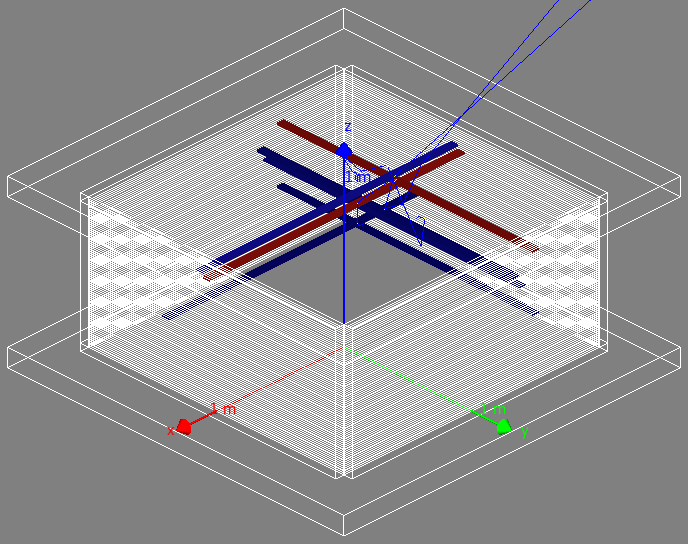
\includegraphics[width=0.7\linewidth]{Chapter4/Figs/Raster/simultaedIbdEvent.png}
 \captionof{figure}{A simulated inverse $\beta$ decay event in GEANT4 in the upgraded detector with 70 layers and shielding around the outside of the detector. The delayed component is shown in blue and the prompt component is shown in red. The delayed component hits more bars than the prompt component.} 
 \label{fig:simultaedIbdEvent}
\end{figure} 

\begin{figure}[htbp]
 \centering
 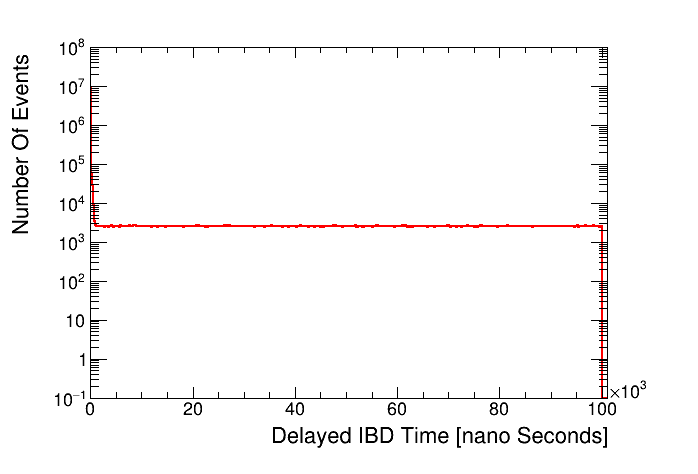
\includegraphics[width=0.7\linewidth]{Chapter4/Figs/Raster/delayedIbdTimes.png}
 \captionof{figure}{The time taken for the neutron from the simulated $\bar{\nu_e}$ inverse $\beta$ decay event to thermilise and be absorbed by the Gadolinium sheets in the simulated VIDARR detector. The tail is extremely long, lasting 1E5\,ns (100\,$\mu$) after the initial peak.} 
 \label{fig:delayedIbdTimes}
\end{figure} 

\begin{figure}[htbp]
 \centering
 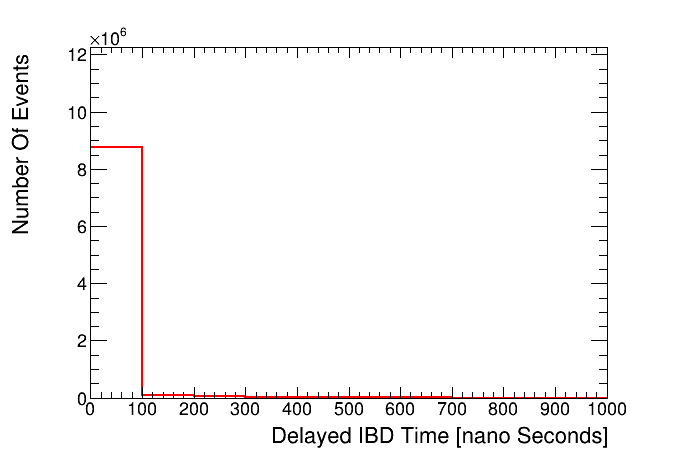
\includegraphics[width=0.7\linewidth]{Chapter4/Figs/Raster/delayedIbdTimesZoom.png}
 \captionof{figure}{Figure \ref{fig:delayedIbdTimes} but with the x axis restricted to 1000\,ns and the y axes no longer on a log scale. This is done to show that above 99.9\,\% of the events are captured before 100\,ns.} 
 \label{fig:delayedIbdTimesZoom}
\end{figure} 

\section{Modelling The Mass Increase}
The number of layers in the prototype detector was 49 out of a possible 70 the upgrade will therefore add $\sim$ 43\,\% additional mass into the detector compared to the prototype. In reality out of a possible 1862 channels in the prototype only 1793 were instrumented due to limitations in securing enough parts. Never the less the simulation will focus on the theoretical maximum number of bars in both cases for the sake of simplicity. As can be seen from figure \ref{fig:prototypeMeasumentFlux} there is an expectation of $\sim$ 200 $\Bar{\nu_e}$ a day and so from the upgraded detector it is reasonable to assume a rate of $\sim$ 300 $\Bar{\nu_e}$ a day with the additional mass. But in addition the quality of each event will also improve as more of the energy from the 8\,MeV $\gamma$ cascade is kept within the bounds of the detector. The amount of energy deposited in the detector will be considered the ``containment'' of the cascade where a containment of 100\,\% would mean 100\,\% of the energy is deposited in the detector. And as figure \ref{fig:containment_comparison} shows the quality of the containment improves with more mass. %In figure \ref{fig:containment_comparison} it can be seen that the quality of the containment increases when the additional mass has been added. 

\begin{figure}[htbp]
 \centering
 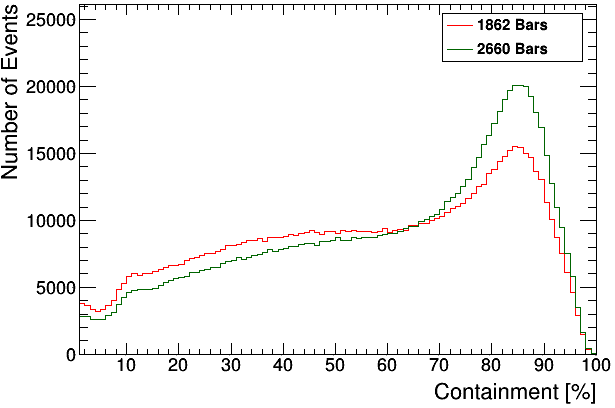
\includegraphics[width=0.7\linewidth]{Chapter4/Figs/Raster/year1Plots/containment_Energy.png}
 \captionof{figure}{Quality of the containment of event energy in the 1862 bars detector and the 2660 bars detector where the containment is defined as the percentage of $\gamma$ cascade reconstructed energy compared to the $\gamma$ cascade generated energy.\hl{this plot needs to be remade with the dicebox}}
 \label{fig:containment_comparison}
\end{figure} 

When simulating e$^-$s and e$^+$s with 0\,MeV -- 10\,MeV kinetic energy the amount of energy contained inside is $\sim$ 100\,\% but slowly decreases as the energy increases. The amount of energy generated (E$_\textrm{{gen}}$) verses the energy deposited  (E$_\textrm{{Dep}}$) for these two particles is shown in figure \ref{fig:recon_gen_ele_pos} contains the energy of charged particles, even small mass particles such as e$^-$ and e$^+$. Then e$^+$ particles are simulated from 1\,MeV -- 10\,MeV to determine efficiencies in figure \ref{fig:2000_3000_p_secs} for both 1862 bars (figure \ref{subFig:2000_p_sec}) and 2660 bars (figure \ref{subFig:3000_p_sec}) above a 0.1\,MeV threshold. In both cases the efficiency doesn't fall below 99\,\% for positrons this is due to the fact that positrons typically don't escape the detector without depositing $>$ 0.1\,MeV in at least a single bar. As such e$^+$ efficiencies don't significantly improve with the mass increase but are extremely high regardless.  

\begin{figure}[htbp]
 \centering
 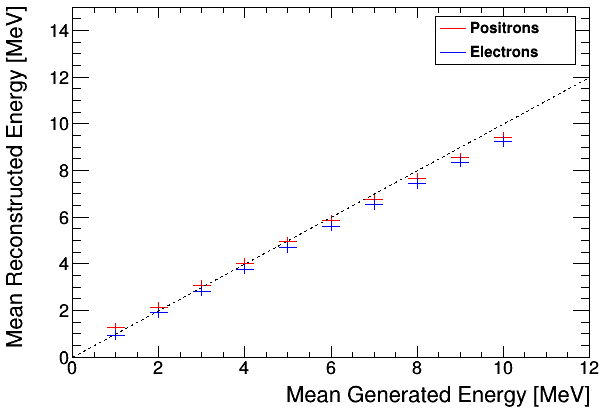
\includegraphics[width=0.7\linewidth]{Chapter4/Figs/Raster/year1Plots/Recon_vs_gen_e-_e+.png}
 \captionof{figure}{Energy response of the simulated detector for both electrons and positrons in the full detector in comparison to E$_\textrm{{dep}}$ = E$_\textrm{{gen}}$. The positron's annihilation $\gamma$s causes E$_\textrm{{dep}}$ $>$ E$_\textrm{{dep}}$ at low generated energies. Deposited error O $\sim$ $10^{-3}$\,MeV  and generated error O $\sim$ $10^{-8}$\,MeV, neither shown as they are both too small to be visible \hl{produce this both 1862 bars and 2660 bars and update axis}.}%~can be used as a kind of place holder in latex
 \label{fig:recon_gen_ele_pos}
\end{figure} 

\begin{figure}[htbp]
\centering
\begin{subfigure}{.5\textwidth}
  \centering
  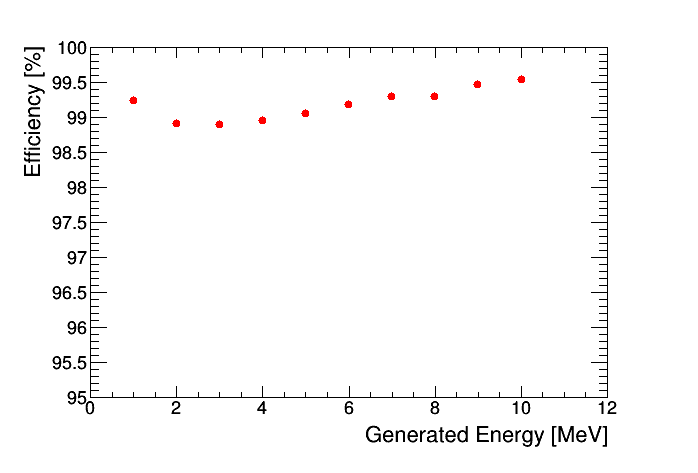
\includegraphics[width=\linewidth]{Chapter4/Figs/Raster/year1Plots/2000_1-10MeV_sec_p_spread_run.png}
  \captionsetup{width=.9\linewidth}
  \caption{Positrons hit efficiencies in 1862 barred detector $\sim$ 99\,\% of positrons are detected.}
  \label{subFig:2000_p_sec}
\end{subfigure}%
\begin{subfigure}{.5\textwidth}
  \centering
  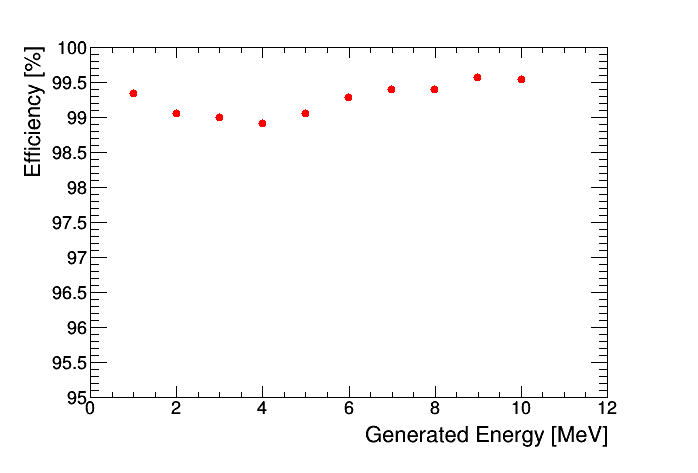
\includegraphics[width=\linewidth]{Chapter4/Figs/Raster/year1Plots/3000_1-10MeV_sec_p_spread_run.png}
  \captionsetup{width=.9\linewidth}
  \caption{Positrons hit efficiencies in 2660 barred detector $\sim$ 99\,\% of positrons are detected.}
  \label{subFig:3000_p_sec}
\end{subfigure}
\caption{Positron hit efficiencies for the original 1862 barred detector and the upgraded 2660 barred detector above a 0.1\,MeV threshold both have $\sim$ 99\,\% efficiencies are similar in both errors are too small to be shown Generated energy O $\sim$ $10^{-8}$ efficiency error O $\sim$ $10^{-3}$.}
\label{fig:2000_3000_p_secs}
\end{figure}

\section{Modelling $\mu$}
$\mu$ are high energy particles with high penetration. As a result atmospheric $\mu$ act as minimally ionising particles (MIPs) this means that the amount of energy deposited per cm ($dE/dx$) is largely independent of the generated energy in-between 100[MeV/$c$] -- 100[GeV/$c$] (see figure \ref{fig:pdg_MuonMomentumStopping}). Whilst figure \ref{fig:pdg_MuonMomentumStopping} shows many different effects and when they take effect for $\mu$ this figure only shows the effect incident on a copper surface. The detector is not comprised of Cu it is comprised of hydrocarbons, specifically polythene. By mass polythene is more C than H so by looking at the momentum ranges 0.1\,GeV/$c$ to 100\,GeV/$c$ in figure \ref{fig:pdg_dedx_gcm2} it is reasonable to assume a dE/dx of $\sim$ 2 g$^{-1}$ cm$^2$ for $\mu$ on C. 

\begin{figure}[htbp]
 \centering
 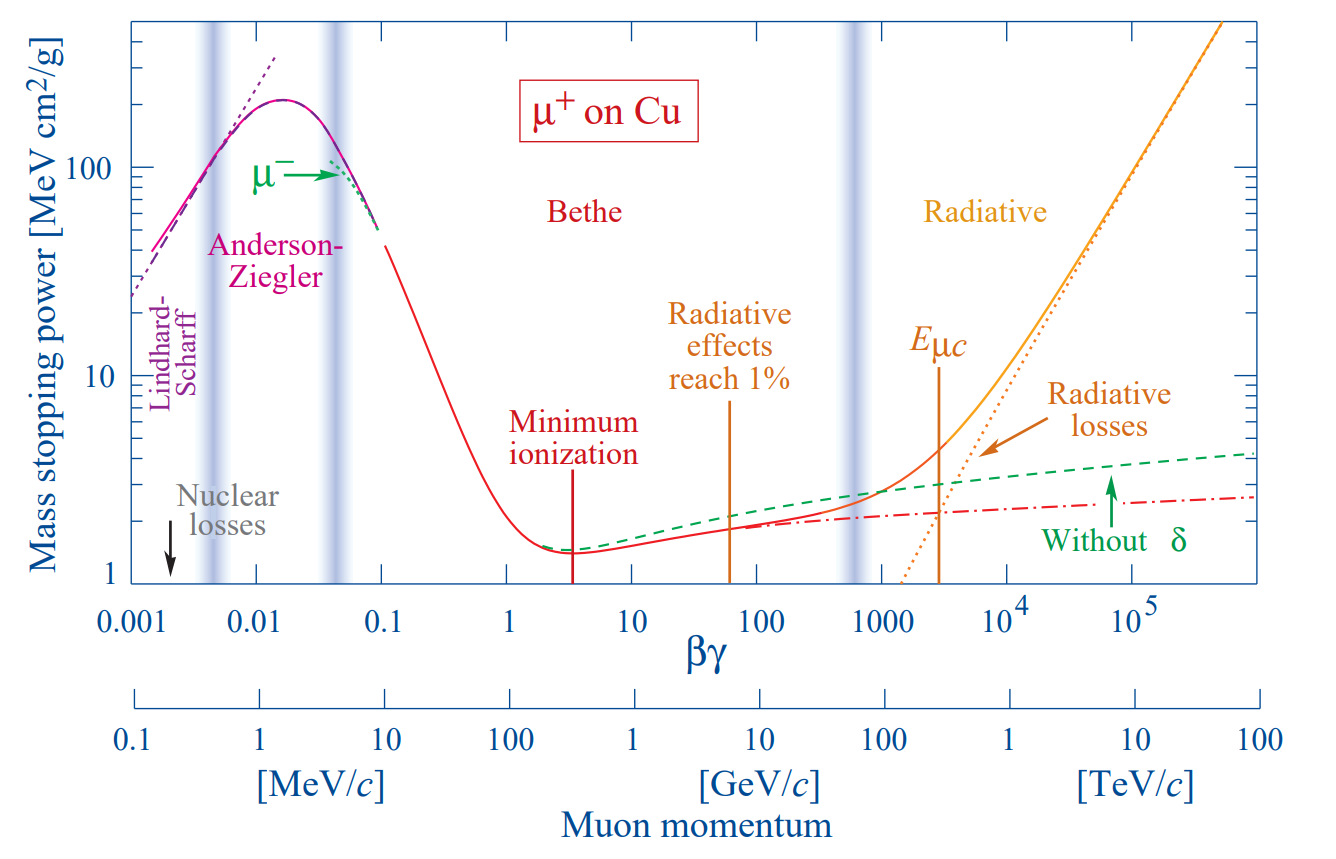
\includegraphics[width=1.0\linewidth]{Chapter4/Figs/Raster/pdg_MuonMomentumStopping.png}
 \captionof{figure}{Mass stopping power for positive $\mu$ in copper as a function of $\beta$ $\gamma$ = $\rho/Mc$ over nine orders of magnitude in momentum (12 orders of magnitude in kinetic energy). From \cite{Olive_2014}.} 
 \label{fig:pdg_MuonMomentumStopping}
\end{figure}

\begin{figure}[htbp]
 \centering
 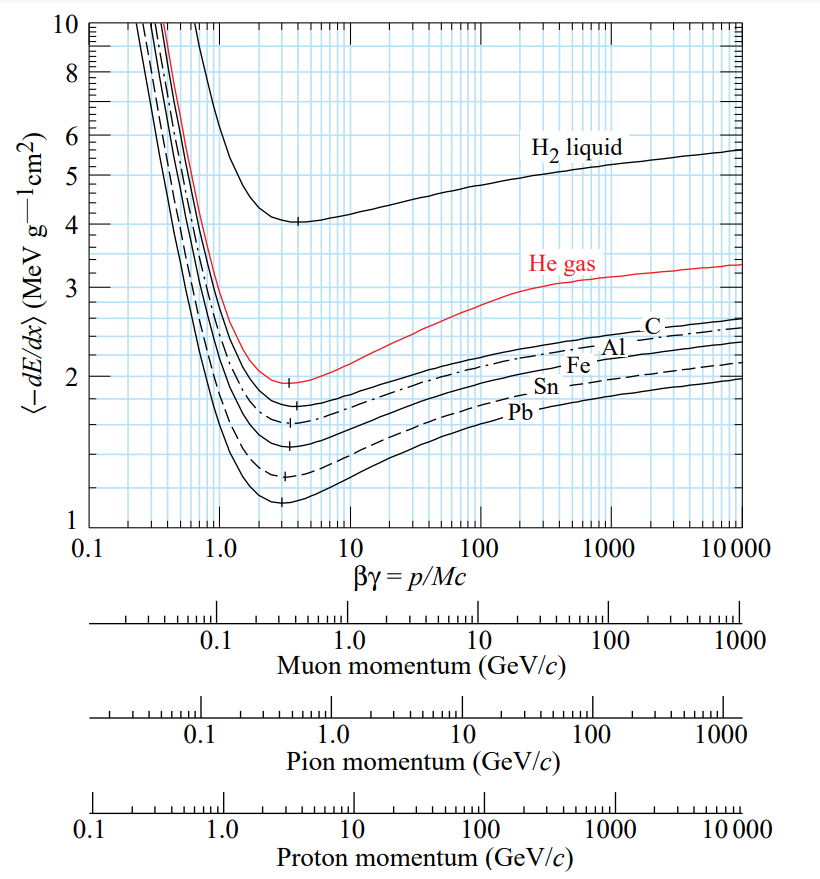
\includegraphics[width=0.7\linewidth]{Chapter4/Figs/Raster/pdg_dedx_gcm2.png}
 \captionof{figure}{Mean energy loss rate in liquid (bubble chamber) hydrogen, gaseous
helium, carbon, aluminum, iron, tin, and lead. Radiative effects, relevant for
$\mu$ and $\pi$, are not included. From \cite{Olive_2014}.} 
 \label{fig:pdg_dedx_gcm2}
\end{figure}

By simulating a single scintillating bar of dimensions 4\,cm $\times$ 152\,cm $\times$ 1\,cm (X,Y,Z) and firing a $\mu$ directly down in the Z plane it is possible to measure the $dE/dx$ in simulation. The energy deposition approximates $dE/dx$ in units of MeV/cm. By simulating the generated kinetic $\mu$ energy from 0.1\,MeV -- 250\,MeV in figure \ref{fig:muon_0_250} the mean energy deposition settles to MIP levels of $\sim$ 2 MeV/cm between 100\,MeV -- 200\,MeV. The CRY library \cite{ieee_cry_2007} can then be used to approximate the expected energies from cosmic $\mu$ which is shown in figure \ref{fig:keMevCryMuons}. In figure \ref{fig:keMevCryMuons} > 99\,\% of the $\mu$ particles produced by the CRY library are between 0.1\,GeV -- 40\,GeV. This coupled with figures \ref{fig:pdg_MuonMomentumStopping} and \ref{fig:pdg_dedx_gcm2} make it reasonable to assume that > 99\,\% of the expected $\mu$ distribution will be MIP like in its behaviour. The distribution for the energy loss of fast particles by ionisation was quantified by Landau in 1944 \cite{landau1944energy}. The Landau distribution represents the energy deposited and is characterised by a sharp peak with a long tail. When simulating high energy $\mu$ this Landau distribution is visible in the events that deposit in the bar which is shown by figure \ref{fig:mev_per_cm_muons}. The offset for measuring the value of dE/dx is shown in figure \ref{fig:lengthAndSideViewBarMuon}. Using the points previously discussed it is reasonable to assume that $>$ 99\,\% of events will have a Landau distribution. %and can be seen in the simulated bar results in figure \ref{fig:mev_per_cm_muons}. More than 99\,\% of the $\mu$ distribution will have the Landau distribution shown in figure \ref{fig:mev_per_cm_muons}. 

\begin{figure}[htbp]
 \centering
 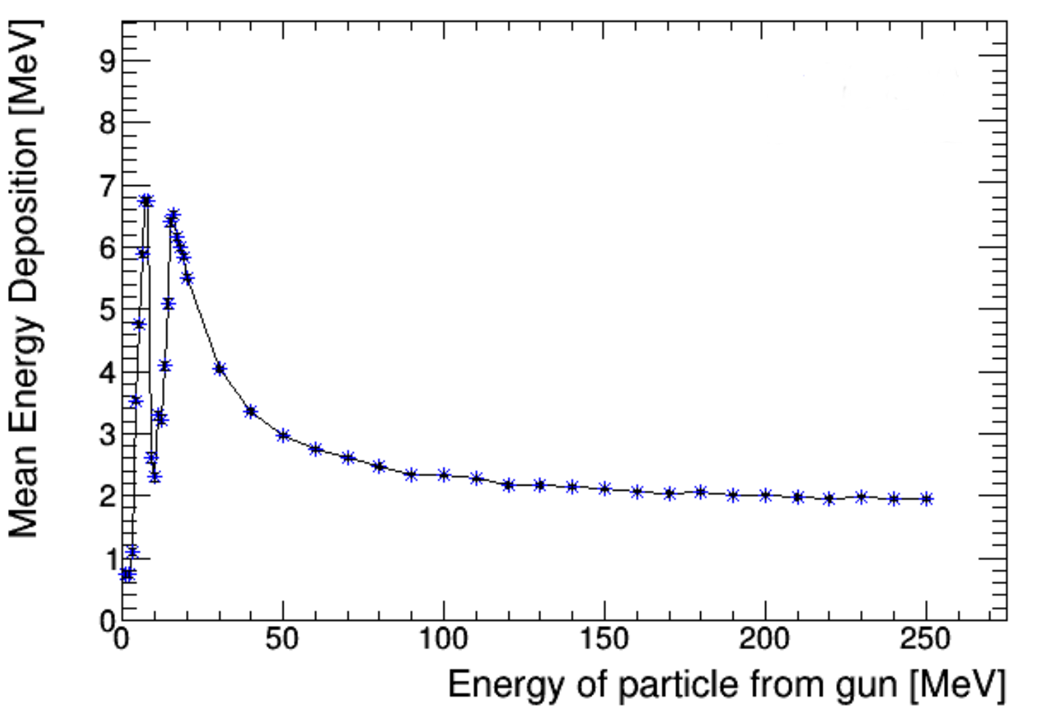
\includegraphics[width=0.7\linewidth]{Chapter4/Figs/Raster/year1Plots/Muon_TiO2_med_eng.png}
 \captionof{figure}{$\mu$ mean energy deposition in active component of the single bar, the sharp decrease in the energy deposited and varying deposition below 20\,MeV was due to the TiO$_2$ coating absorbing $\mu$ at lower energies.} 
 \label{fig:muon_0_250}
\end{figure}

\begin{figure}[htbp]
 \centering
 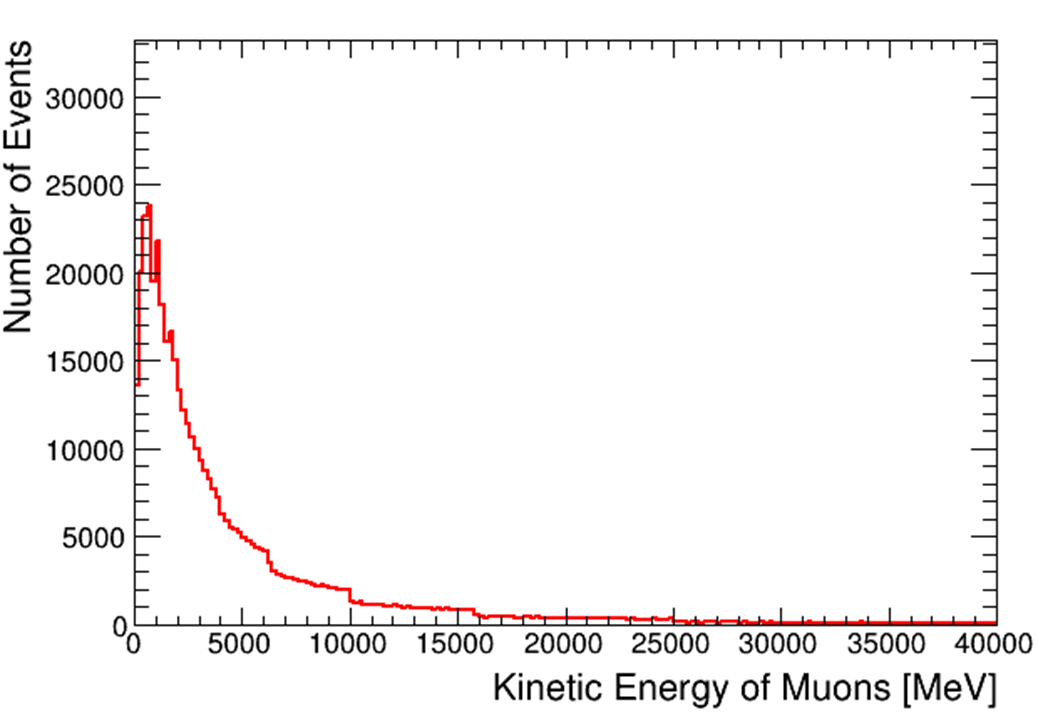
\includegraphics[width=0.7\linewidth]{Chapter4/Figs/Raster/keMevCryMuons.png}
 \captionof{figure}{Generated kinetic energy $\mu$ particles using the CRY library \cite{ieee_cry_2007} at sea level with latitude 53$^\circ$ (Liverpool's latitude) and date: 01 -- March -- 2021. 99\,\% + of generated $\mu$ particles are between 0.1\,GeV (100\,MeV) and 40\,GeV (40000\,MeV) kinetic energy.} 
 \label{fig:keMevCryMuons}
\end{figure}

\begin{figure}[htbp]
 \centering
 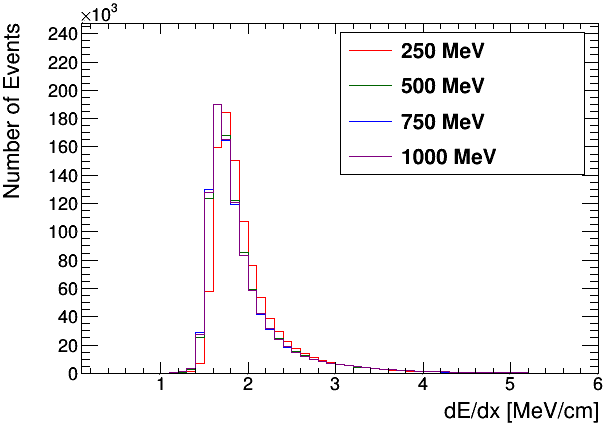
\includegraphics[width=0.7\linewidth]{Chapter4/Figs/Raster/year1Plots/muons_per_mev_cm.png}
 \captionof{figure}{dE/dx of $\mu$ through single plastic bar assuming a density of plastic of 1\,g\,cm$^{-3}$. Mearuemnts for plastic are similar to carbon. For carbon $\sim$ 2\,MeV\,cm$^{-1}$ is expected for dE/dx {\cite{Olive_2014}. Mean dE/dx for 250\,MeV, 500\,MeV, 750\,MeV, 1000\,MeV are respectively 1.9907 $\pm$  0.0005\,MeV\,cm$^{-1}$, 1.9387 $\pm$  0.0005\,MeV\,cm$^{-1}$, 1.9374 $\pm$  0.0005 MeV\,cm$^{-1}$, 1.9407 $\pm$  0.0005 MeV\,cm$^{-1}$.\\}}
 \label{fig:mev_per_cm_muons}
\end{figure}

As mentioned before the CRY library is very useful as it contains a large amount of relevant physics information with the latest version being 1.7 produced in 2012 \cite{hagmann2012cosmicCry}. The CRY library splits up the directions in the x,y and z by using cosine directions u (see equation\ref{equ:cos_u}), v (see equation \ref{equ:cos_v}) and w (see equation \ref{equ:cos_w}) respectively. However, whilst the generated cosine direction for u and v were very fine the binning for cosine w was coarse. As a result an 8 dimensional polynomial function was fitted to the cosine w distribution in figure \ref{fig:Cry_GeneratedFit} to smooth out the distribution. The improvement to the distribution can be seen in figure \ref{fig:CrySmoothingCosTheta} where the finer binning of the cosine direction w in figure \ref{subFig:CrySmoothingCosine} leads to a smoother more accurate $\theta$ distribution in figure \ref{subFig:CrySmoothingTheta}. 

\begin{equation}
\alpha = \cos{u} = \frac{v_x}{\sqrt{v_x^2+v_y^2+v_z^2}}
\label{equ:cos_u}
\end{equation}

\begin{equation}
\beta = \cos{v} = \frac{v_y}{\sqrt{v_x^2+v_y^2+v_z^2}}
\label{equ:cos_v}
\end{equation}

\begin{equation}
\gamma = \cos{w} = \frac{v_z}{\sqrt{v_x^2+v_y^2+v_z^2}}
\label{equ:cos_w}
\end{equation}

\begin{figure}[htbp]
 \centering
 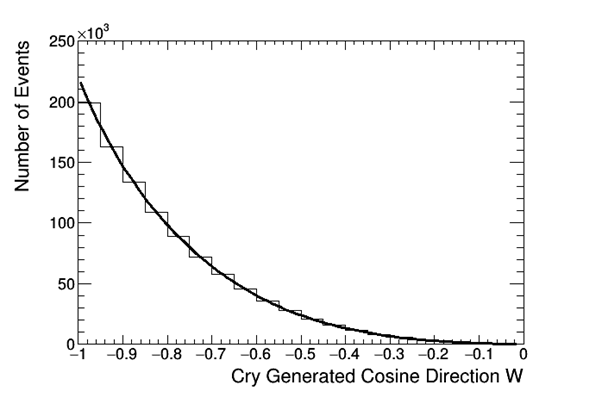
\includegraphics[width=0.7\linewidth]{Chapter4/Figs/Raster/CryPlots/Cry_GeneratedFit.png}
 \captionof{figure}{The generated angles for cosine direction W (z axis) from the CRY library \cite{hagmann2007cosmic} for 1 million particles. Binning in CRY is 0.05 so an 8 dimensional polynomial was fitted to smooth the distribution.}
 \label{fig:Cry_GeneratedFit}
\end{figure}

\begin{figure}[htbp]
\centering
\begin{subfigure}{.5\textwidth}
  \centering
  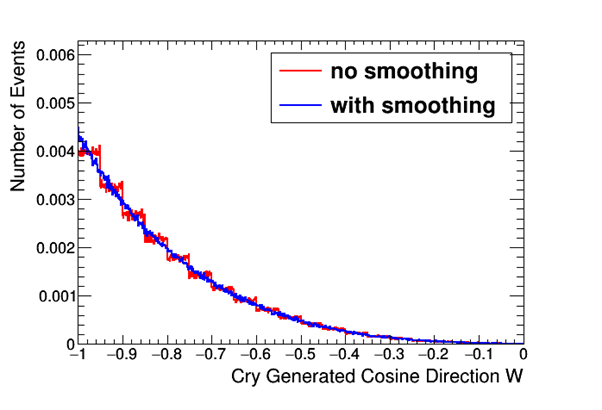
\includegraphics[width=\linewidth]{Chapter4/Figs/Raster/CryPlots/CrySmoothingCosine.png}
  \captionsetup{width=.9\linewidth}
  \caption{Smoothed distribution for the cosine direction in W compared to the originally generated CRY distribution.}
  \label{subFig:CrySmoothingCosine}
\end{subfigure}%
\begin{subfigure}{.5\textwidth}
  \centering
  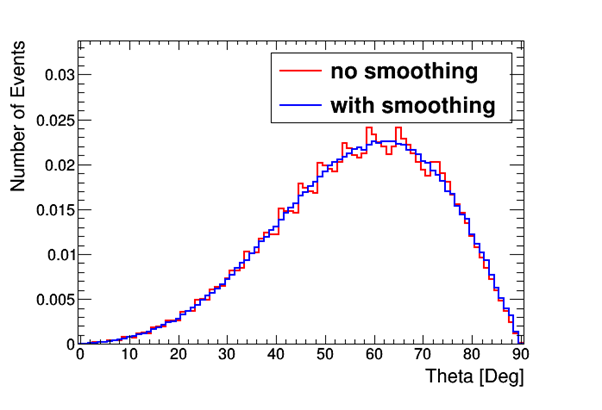
\includegraphics[width=\linewidth]{Chapter4/Figs/Raster/CryPlots/CrySmoothingTheta.png}
  \captionsetup{width=.9\linewidth}
  \caption{Smoothed distribution of $\theta$ compared to the originally generated CRY distribution.}
  \label{subFig:CrySmoothingTheta}
\end{subfigure}
\caption{How the smoothing effects the CRY distribution in Cos W and $\theta$. The nonphysical peaks seen in the non-smoothed $\theta$ distribution are a direct result of CRY's coarse binning in $\theta$.}
\label{fig:CrySmoothingCosTheta}
\end{figure}

Now the $\theta$ distribution has been smoothed out accordingly the cosmic $\mu$ particles need to be back projected. Back projection is where positions that CRY generates (see figure \ref{fig:cryxm_vs_cryym}) is taken as a ``target'' and then the $\phi$ values (a flat distribution between 0 -- 360$^\circ$) and smoothed $\theta$ values (see figure \ref{subFig:CrySmoothingTheta}) are used to project backwards to a point for a given radius. The larger the back projection radius the more accurate the simulation but the more computationally intensive it becomes. A back projection of 100\,m is a reasonable approximation to simulate all incoming side on and top down events. Figure \ref{fig:BackProjectionXY} shows how this looks in the x and y from a top down perspective. The ``halo'' in figure \ref{fig:BackProjectionXY} is a result of the $\theta$ distribution seen in figure \ref{subFig:CrySmoothingTheta}. The rest of the simulated dome can be seen in figure \ref{fig:BackProjection_XZ_YZ} where the XZ and YZ distributions are very similar to each other. 

\begin{figure}[htbp]
 \centering
 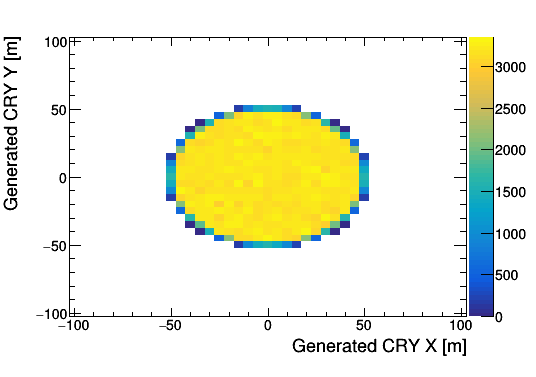
\includegraphics[width=0.7\linewidth]{Chapter4/Figs/Raster/CryPlots/cryxm_vs_cryym.png}
 \captionof{figure}{Generated CRY X and Y positions in the simulation. A circle has been cut out of the generated square to give a flat $\phi$ distribution. All particles in CRY are generated at Z = 0.} 
 \label{fig:cryxm_vs_cryym}
\end{figure}

\begin{figure}[htbp]
 \centering
 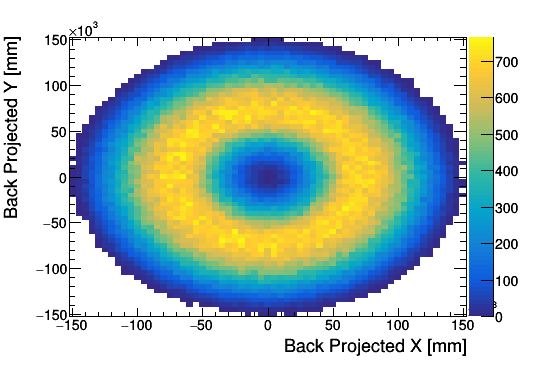
\includegraphics[width=0.7\linewidth]{Chapter4/Figs/Raster/CryPlots/BackProjectionXY.png}
 \captionof{figure}{Back projection of 100\,m in the X and Y plane for the CRY library this represents the starting position for each particle generated in X and Y.} 
 \label{fig:BackProjectionXY}
\end{figure}

\begin{figure}[htbp]
\centering
\begin{subfigure}{.5\textwidth}
  \centering
  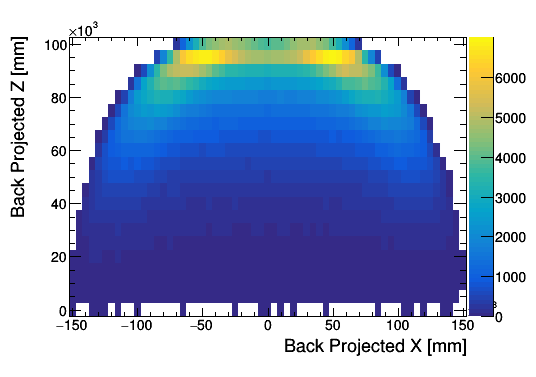
\includegraphics[width=\linewidth]{Chapter4/Figs/Raster/CryPlots/BackProjectionXZ.png}
  \captionsetup{width=.9\linewidth}
  \caption{Starting positions for generated CRY distribution using a back projection of 100\,m in X and Z.}
  \label{subFig:BackProjectionXZ}
\end{subfigure}%
\begin{subfigure}{.5\textwidth}
  \centering
  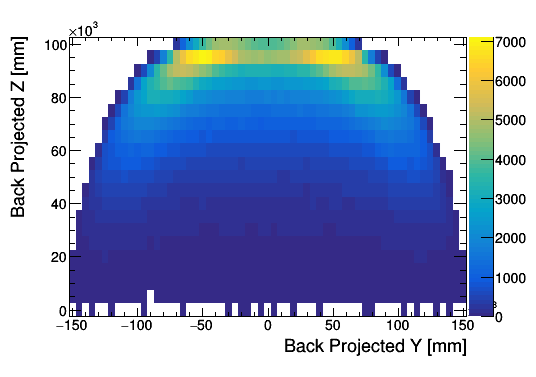
\includegraphics[width=\linewidth]{Chapter4/Figs/Raster/CryPlots/BackProjectionYZ.png}
  \captionsetup{width=.9\linewidth}
  \caption{Starting positions for generated CRY distribution using a back projection of 100\,m in Y and Z.}
  \label{subFig:BackProjectionYZ}
\end{subfigure}
\caption{Starting positions for the generated CRY distribution for XZ and YZ with a back projection of 100\,m.}
\label{fig:BackProjection_XZ_YZ}
\end{figure}

The impact of back projection is relatively small when looking at where the particles cross the z Axis. As shown in figure \ref{fig:Crossed_atZ_XY_AndShort} when comparing a back projection of 1\,cm (figure \ref{subFig:CrossedZAxisShort}) to 100\,m (figure \ref{subFig:Crossed_atZ_XY}) both reproduce the circular distribution seen in figure \ref{fig:cryxm_vs_cryym} there is more scattering with more back projection but this a suitable trade off for vastly more accurate tracks. 

\begin{figure}[htbp]
\centering
\begin{subfigure}{.5\textwidth}
  \centering
  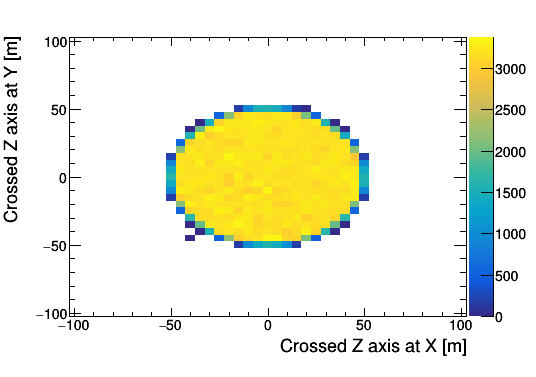
\includegraphics[width=\linewidth]{Chapter4/Figs/Raster/CryPlots/CrossedZAxisShort.png}
  \captionsetup{width=.9\linewidth}
  \caption{Where the CRY distribution crosses the Z axis with only 1\,cm back projection.}
  \label{subFig:CrossedZAxisShort}
\end{subfigure}%
\begin{subfigure}{.5\textwidth}
  \centering
  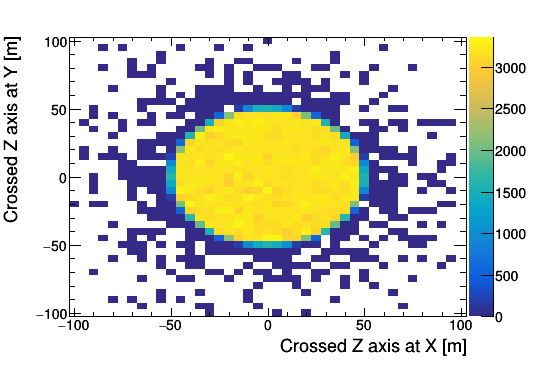
\includegraphics[width=\linewidth]{Chapter4/Figs/Raster/CryPlots/Crossed_atZ_XY.png}
  \captionsetup{width=.9\linewidth}
  \caption{Where the CRY distribution crosses the Z axis after back projected 100\,m.}
  \label{subFig:Crossed_atZ_XY}
\end{subfigure}
\caption{How the generated CRY distribution crosses the Z axis with only 1\,cm of back projection vs 100\,m of back projection. When world environment in GEANT4 is G4 Galactic}
\label{fig:Crossed_atZ_XY_AndShort}
\end{figure}

In addition atmospheric effects need to be modelled. The atmosphere produces two main effects: it increases particle scattering (see figure \ref{fig:gen-scat_PhiTheta} and it increases the rate of secondaries produced (see figure \ref{fig:CRY_rates}). The CRY simulation takes the atmosphere into account \cite{hagmann2007monteCry} but only produces the particles that cross the Z axis at z = 0. As a result the secondaries produced by GEANT4 are also simulated by CRY thus resulting in some secondary particles being ``double simulated.'' This effect is most visible in figure \ref{fig:CRY_rates} where the rates in simulated air are overall $\sim$ 25\,\% higher than in a low density galactic environment. However the paths of these particles are more accurate in the air and the secondaries produced inside a detector still need to be taken into account. For the most accurate cosmic modelling the air should be used whilst killing all secondaries that occur in the air i.e outside the detector. However, due to time constraints this was unable to be added to the simulation. \hl{I would like to change this if there's sufficient time left...}.

\begin{figure}[htbp]
\centering
\begin{subfigure}{.5\textwidth}
  \centering
  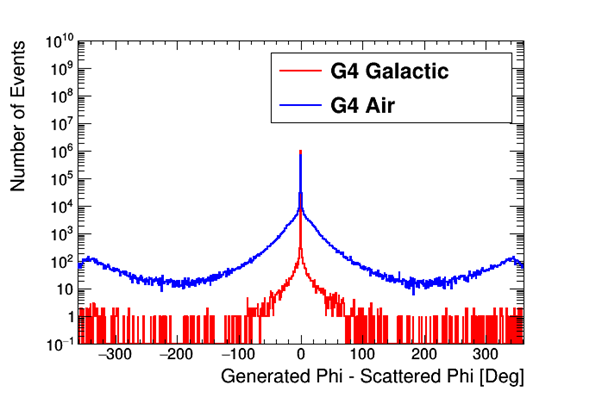
\includegraphics[width=\linewidth]{Chapter4/Figs/Raster/CryPlots/genPhi-scatPhi.png}
  \captionsetup{width=.9\linewidth}
  \caption{How the Generated $\phi$ - scattered $\phi$ varies for air and galactic world material in GEANT4.}
  \label{subFig:genPhi-scatPhi}
\end{subfigure}%
\begin{subfigure}{.5\textwidth}
  \centering
  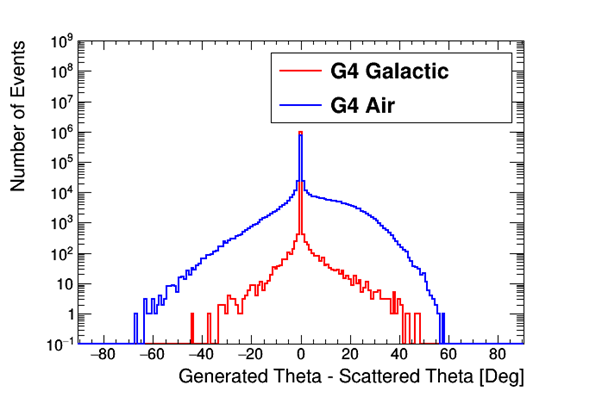
\includegraphics[width=\linewidth]{Chapter4/Figs/Raster/CryPlots/genTheta-scatTheta.png}
  \captionsetup{width=.9\linewidth}
  \caption{How the Generated $\theta$ - scattered $\theta$ varies for air and galactic world material in GEANT4.}
  \label{subFig:genTheta-scatPhi}
\end{subfigure}
\caption{How the scattering in $\phi$ and $\theta$ is effected by world material in GEANT4. Scattering is much more realistic when using G4 Air.}
\label{fig:gen-scat_PhiTheta}
\end{figure}

\begin{figure}[htbp]
 \centering
 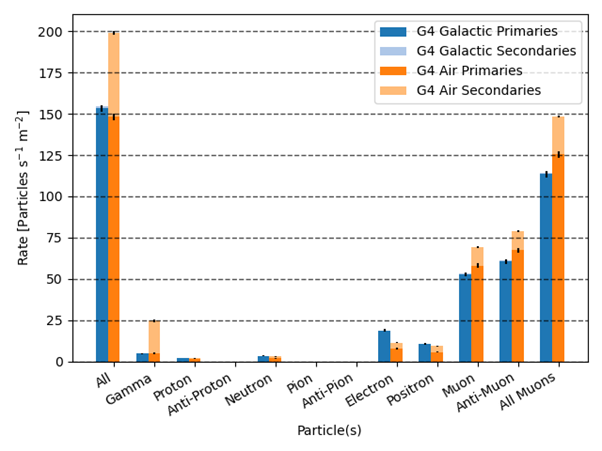
\includegraphics[width=0.8\linewidth]{Chapter4/Figs/Raster/CryPlots/CRY_rates.png}
 \captionof{figure}{How the rates vary depending on the world material in GEANT4. For Galactic world materials secondary production is minimal. The rates are most accurate for Galactic world material but the paths will be more accurate for Air. Measured from a PVT block of 1\,m $\times$ 1\,m $\times$ 1\,cm to approximate particles s$^{-1}$ m$^{-2}$.} 
 \label{fig:CRY_rates}
\end{figure}

\section{Modelling TiO$_2$ Coating}
The plastic scintillating bars of the VIDARR detector are extruded at Fermilab and have been used in other experiments such as the T2K ND280 ECAL \cite{Allan_2013} Miner$\nu$a \cite{aliaga2014design} and in Mu2e as a cosmic ray veto \cite{Pla-Dalmau2014}. This coating needs to be correctly modelled as it can have a significant impact on heavier particles. An example can be see in figure \ref{fig:lengthAndSideViewBarMuon} which shows how the particles were offset to correctly asses the impact of the TiO$_2$ coating. The effect for less massive particles such as e$^+$ (see figure \ref{fig:positron_TiO2}) is virtually non-existent over the energy range of interest (0 -- 10\,MeV). The effect of the TiO$_2$ coating is more noticeable for $\mu$ however this will only impact stopping $\mu$ with energies < 5\,MeV as seen in figure \ref{fig:muon_TiO2}. A significant effect is seen with protons in figure \ref{fig:proton_TiO2} and this effects all protons between 0 -- 15\,MeV and so for simulation purposes it is important the TiO$_2$ coating is correctly quantified. The TiO$_2$ coating is 15\,\% TiO$_2$ to 85\,\% polythene \cite{aliaga2014design} \cite{Pla-Dalmau2014} with a thickness of 0.25\,mm \cite{Pla-Dalmau2014}. And this is now correctly modelled in the full detector and single bar GEANT4 simulation.

\begin{figure}[htbp]
 \centering
 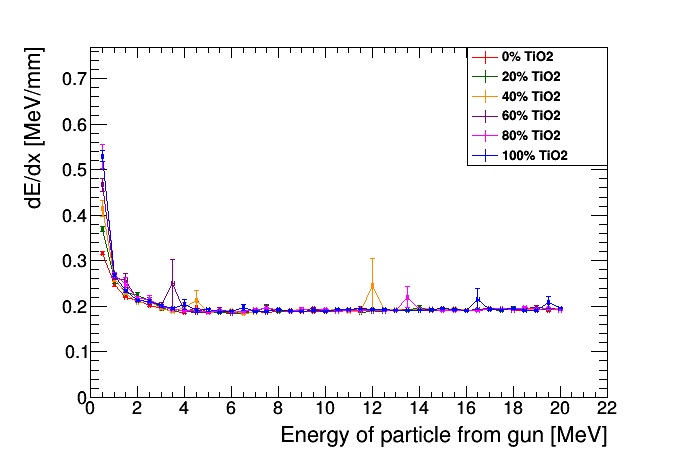
\includegraphics[width=0.7\linewidth]{Chapter4/Figs/Raster/year1Plots/positron_TiO2__.png}
 \captionof{figure}{The average dE/dx for generated positrons deposited in a single bar of scintillator the \% of TiO$_2$ has minimal effect on positrons. The dE/dx occasionally rises due to annihilation $\gamma$s depositing energy.} 
 \label{fig:positron_TiO2}
\end{figure}

\begin{figure}[htbp]
 \centering
 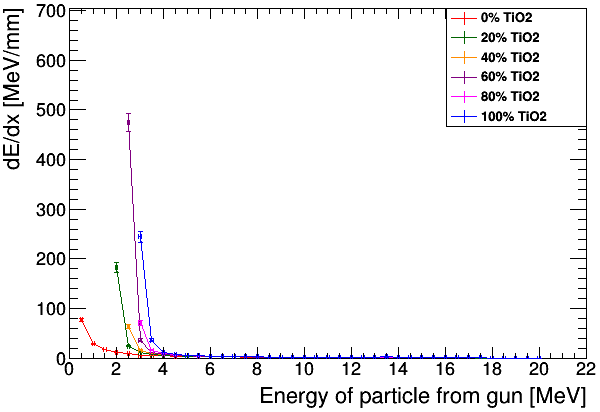
\includegraphics[width=0.7\linewidth]{Chapter4/Figs/Raster/year1Plots/muon_TiO2__.png}
 \captionof{figure}{The average dE/dx for generated cosmic $\mu$ deposited in a single bar of scintillator the \% of TiO$_2$ has some impact on the dE/dx at low energies.} 
 \label{fig:muon_TiO2}
\end{figure}

\begin{figure}[htbp]
 \centering
 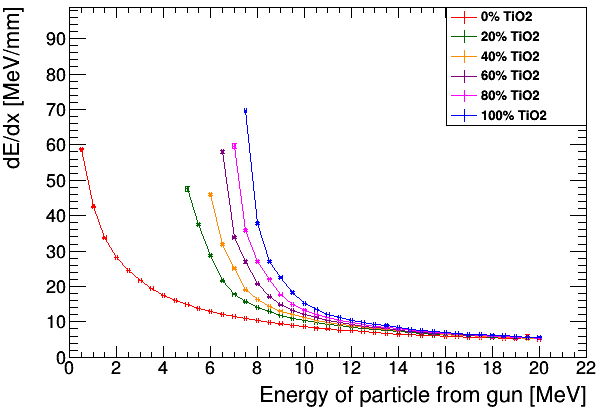
\includegraphics[width=0.6\linewidth]{Chapter4/Figs/Raster/year1Plots/proton_TiO2__.png}
 \captionof{figure}{The average dE/dx for generated protons deposited in a single bar of scintillator the \%  of TiO$_2$ coating has significant impact except towards higher energies.}
 \label{fig:proton_TiO2}
\end{figure}

\begin{figure}[htbp]
\centering
\begin{subfigure}{.5\textwidth}
  \centering
  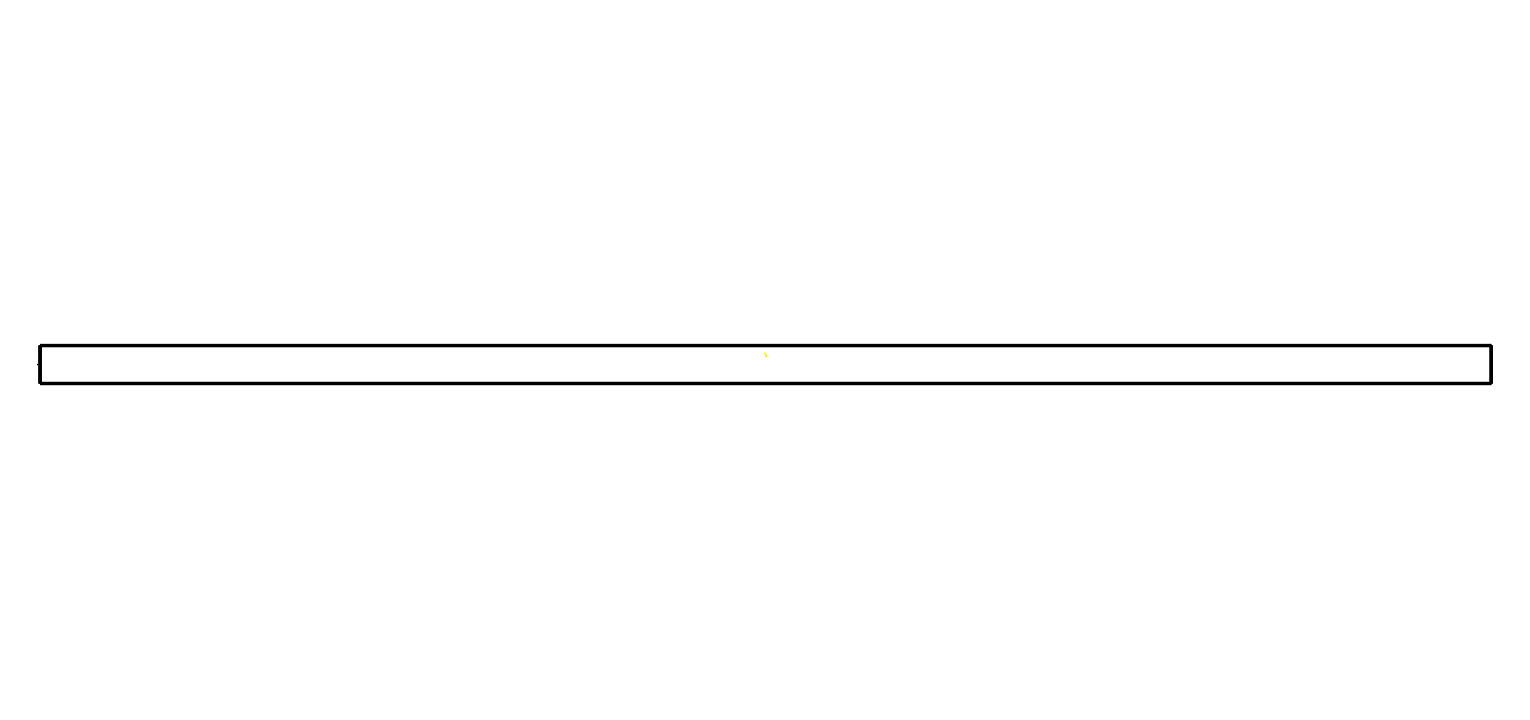
\includegraphics[width=\linewidth]{Chapter4/Figs/Raster/lengthOnViewBarMuon1530By720.png}
  \captionsetup{width=.9\linewidth}
  \caption{Length ways view.}
  \label{subFig:lengthOnViewBarMuon1530Square}
\end{subfigure}%
\begin{subfigure}{.5\textwidth}
  \centering
  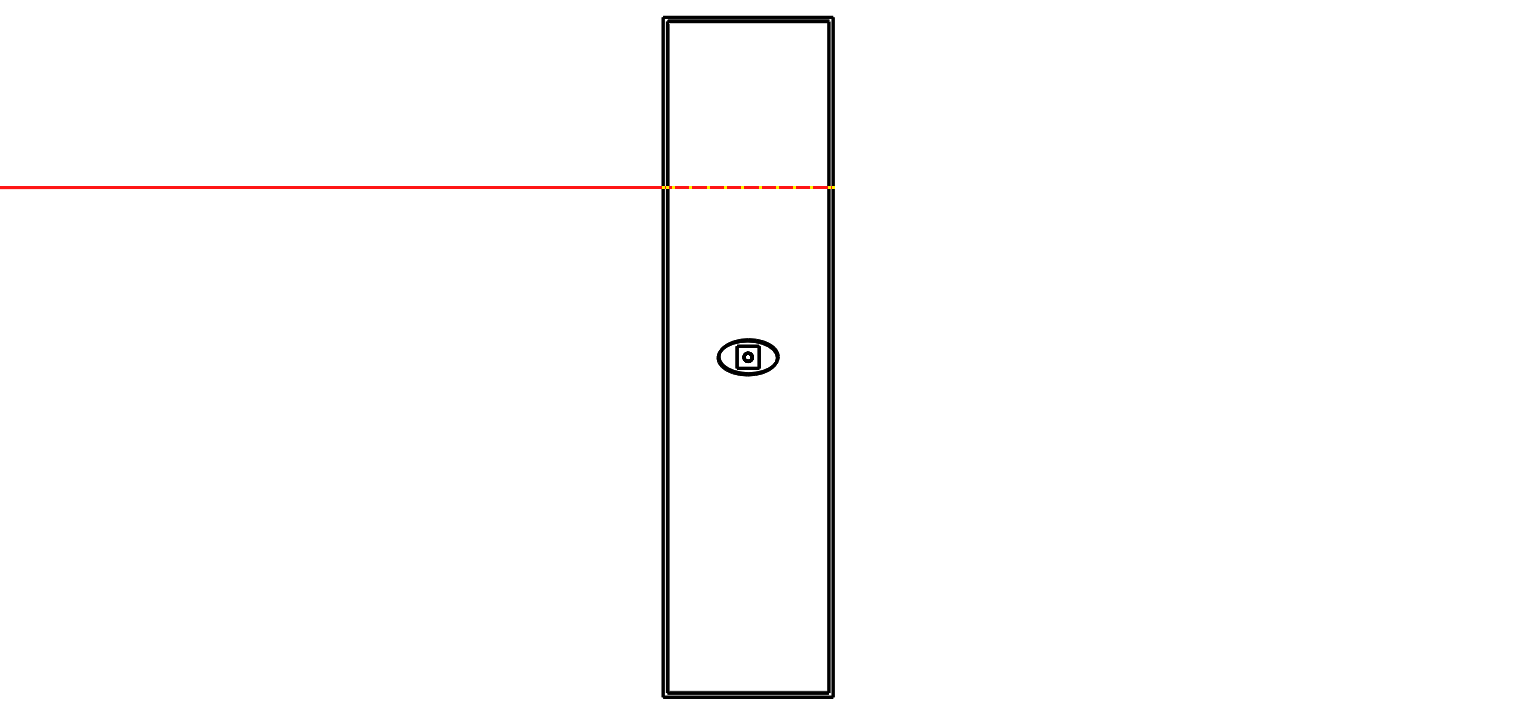
\includegraphics[width=\linewidth]{Chapter4/Figs/Raster/sideOnViewBarMuon1530By720.png}
  \captionsetup{width=.9\linewidth}
  \caption{Side on view.}
  \label{subFig:sideOnViewBarMuon8}
\end{subfigure}
\caption{How a 20\,MeV $\mu$ particle penetrates through the coating and scintillator it is offset to ensure the effect from the TiO$_2$ coating is being correctly observed.}
\label{fig:lengthAndSideViewBarMuon}
\end{figure}

\section{Modelling Attenuation}\label{sec:GEANT4Simulation_ModellingAttenuation}
In order to characterise the physical effects of the detector a test stand was set up by fellow collaborator George Holt. This test stand contained a single plastic scintillating bar where a caesium 137 source was placed at 11 intervals across the bar from which attenuation of the 662\,KeV peak could be measured. This is shown in figure \ref{fig:attenuationPlot} the exponential function (equation \ref{equ:attenuationFunction}) is used by the simulation to produce a data driven model for the light attenuation in the simulation. 

\begin{equation}
P(x) = e^{-x/\lambda}
\label{equ:attenuationFunction}
\end{equation}

\begin{figure}[htbp]
 \centering
 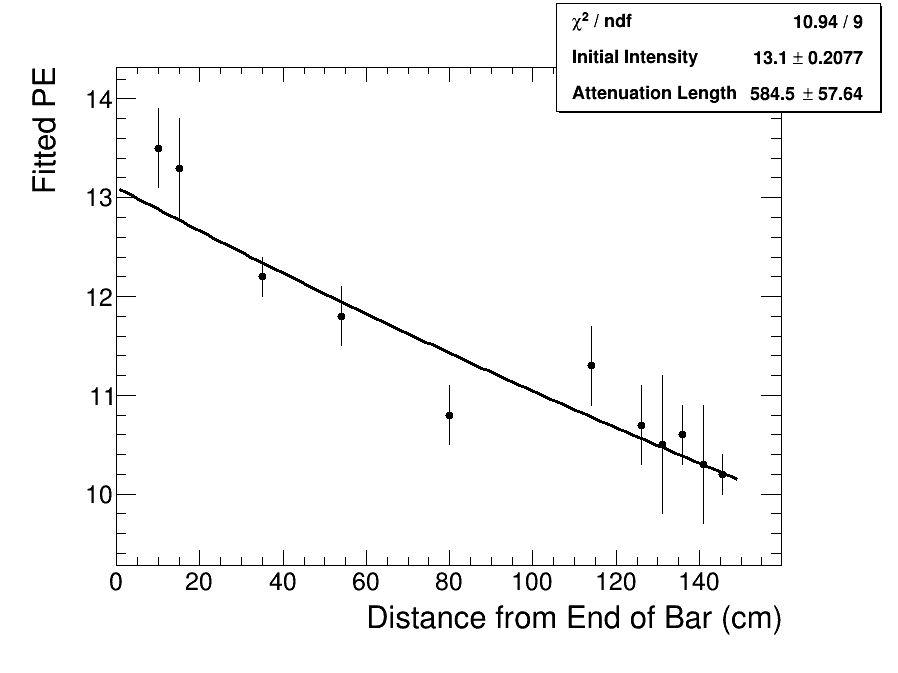
\includegraphics[width=1.0\linewidth]{result_from_attnPlotter.png} 
 \captionof{figure}{The attenuation plot from the single bar test stand produced by George Holt. The attenuation length (amount of bar traversed to lose $\sim$ 63\,\%  of light, $\lambda$ in equation \ref{equ:attenuationFunction}) is 580 $\pm$ 60\,PE/cm. \hl{need to move the box with the stats into the axis/ get rid of it}.} 
 \label{fig:attenuationPlot}
\end{figure}

\section{Modelling Dark Noise}\label{sec:GEANT4Simulation_ModellingDarkNoise}
Another data driven physical effect modelled in the simulation is the dark noise. Depending on temperature MPPCs will emit signals that are due to electronic effects rather than particle measurements. The dark noise was measured at room temperature over a 12 hour period by George Holt. The results in figure \ref{fig:pureDarkNoise} show Photo-electron (PE) peaks in units of mV with peaks for 1\,PE, 2\,PE and 3\,PE being clearly visible at 4.1\,mV, 8.2\,mV, and 12.3\,mV respectively. In order to measure the dark noise an MPPC was put inside a container where no light would reach the sensor. 
\begin{figure}[htbp]
 \centering
 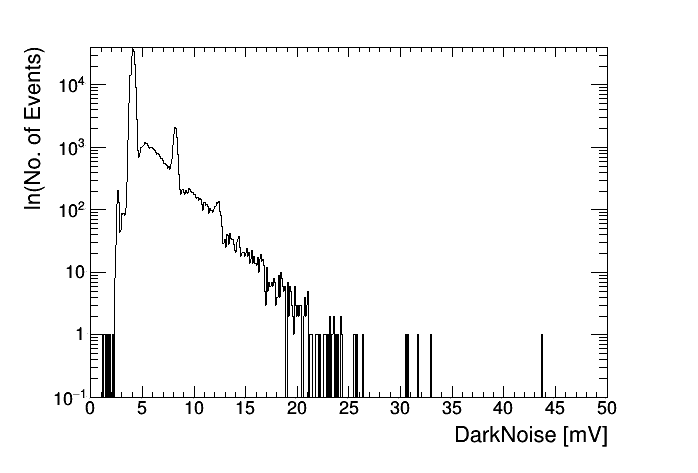
\includegraphics[width=0.8\linewidth]{pureDarkNoise_output.png}
 \captionof{figure}{Dark Noise from the MPPC taken over a period of $\sim$ 12\,hrs, taken by George Holt. The PE peaks for 1\,PE 2\,PE and 3\,PE can be seen at 4.1\,mv, 8.2\,mv and 12.3\,mv respectively. } 
 \label{fig:pureDarkNoise}
\end{figure}

The dark noise has two distinct components: the peaks, and the background surrounding the peaks. The background surrounding the peaks can be modelled using an exponential fit which is done in figure \ref{subFig:expFitOfDark}. The pedestal peak (seen at 3\,mV in figure \ref{fig:pureDarkNoise}) is also removed and an exponential is used past 13.7\,mV (see figure \ref{subFig:fittedDarkNoise}). 
\begin{figure}[htbp]
\centering
\begin{subfigure}{.5\textwidth}
  \centering
  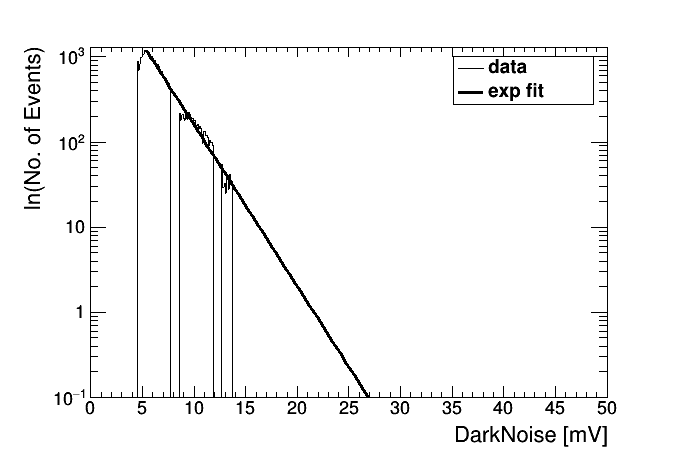
\includegraphics[width=\linewidth]{fit_of_dark_noise.png}
  \captionsetup{width=.9\linewidth}
  \caption{Fit of exponential function using TFit to fit the after-pulsing of the MPPCs}
  \label{subFig:expFitOfDark}
\end{subfigure}%
\begin{subfigure}{.5\textwidth}
  \centering
  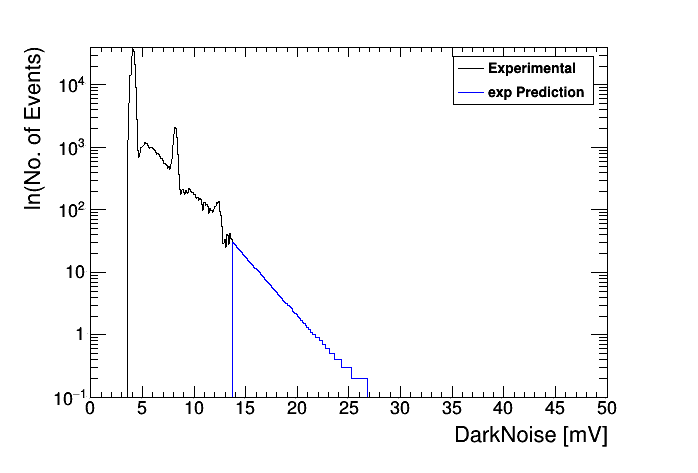
\includegraphics[width=\linewidth]{fittedDarkNoise_output.png}
  \captionsetup{width=.9\linewidth}
  \caption{Fitted exponential past 13.7\,mv once the number of events dropped below 10.}
  \label{subFig:fittedDarkNoise}
\end{subfigure}
\caption{Dark Noise from an MPPC taken over a period of $\sim$ 12\,hrs with an exponential fitted, with a $\chi ^2$ /DOF = 159.748}
\label{fig:fitting_of_non_peak_dark_noise}
\end{figure}

The results from figure \ref{fig:fitting_of_non_peak_dark_noise} can then be used to construct a cumulative probability distribution seen in figure \ref{fig:cumulative_prob_dark}. This probability distribution is what the simulation reads to reconstruct the dark noise distribution. During the simulation a random dice is thrown and that probability is then converted back into a dark noise value which is then assigned to a random bar in the detector. Values past 13.7\,mV use the exponential fit. These events extrapolate directly from the exponential fit instead of reading from the probability distribution for more realistic results. The dark noise produced for 1 bar in simulation for 1E6 events is shown in figure \ref{individualDarkNoiseOld}. 
\begin{figure}[htbp]
 \centering
 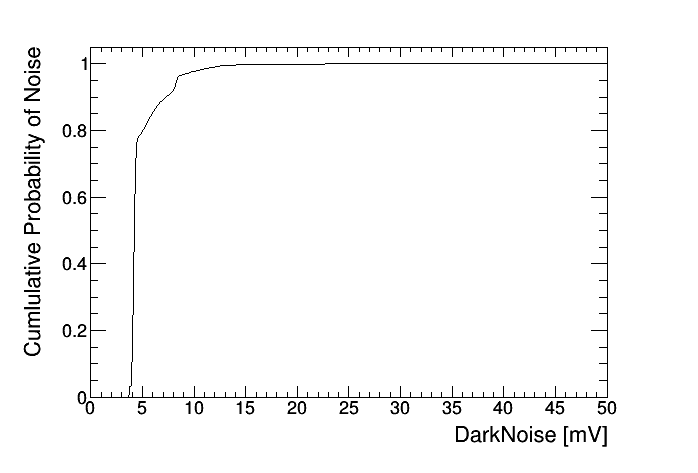
\includegraphics[width=0.8\linewidth]{cumulative_prob_dark_noise.png}
 \captionof{figure}{Cumulative probability of the dark noise, which is converted to a table and then searched using the golden section search} 
 \label{fig:cumulative_prob_dark}
\end{figure}

\begin{figure}[htbp]
 \centering
 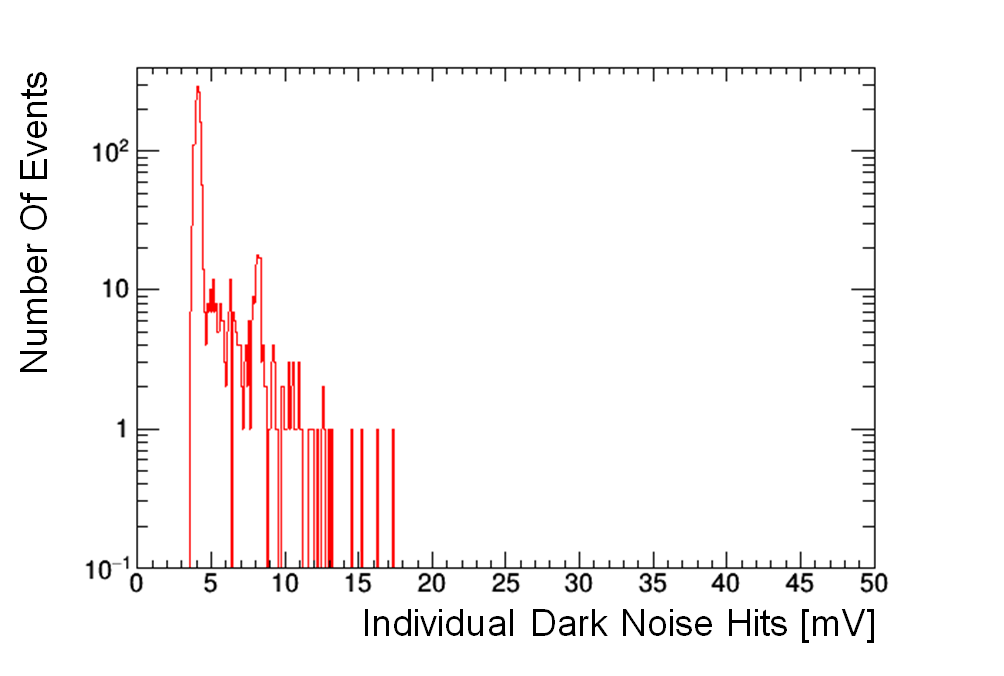
\includegraphics[width=0.8\linewidth]{Chapter4/Figs/Raster/individualDarkNoiseOld.png}
 \captionof{figure}{The dark noise produced for a single bar in simulation with 1E6 events \hl{Planning to do this for more stats and full detector to give a better view of how the distribution looks in simulation}.} 
 \label{fig:individualDarkNoiseOld}
\end{figure}

\section{Modelling Light Emission}\label{sec:GEANT4Simulation_ModellingLightEmission}
In order to measure light for a given amount of scintillating material we need to consider several factors. For organic scintillators the type of particle has a significant effect on the absolute light yield. The response of organic scintillators to charged particles can best be described by a relation between $dL/dx$ the fluorescent energy emitted per unit path length and $dE/dx$ the specific energy loss for the charged particle.  A widely used relation first suggested by Birks \cite{birks_1964} is based on the assumption that a high ionisation density along the track of the particle leads to quenching from damaged molecules and a lowering of  scintillation efficiency. If we assume that the density of damaged molecules along the wake of the particle is directly proportional to the ionisation density we can represent their density by $B(dE/dx)$ where $B$ is a proportionality constant. Birks assumes that some fraction $k$ of these will lead to quenching\cite{knoll_2010}. A further assumption is that in absence of quenching the light yield is proportional to energy loss shown in equation \ref{equ:light_yield_proportional}. In equation \ref{equ:light_yield_proportional} $S$ is the normal scintillation efficiency \cite{birks_1964}. To account for the probability of quenching Birks then writes equation \ref{equ:Birks_formula}. Equation \ref{equ:Birks_formula} is commonly referred to as the Birks formula. The product $kB$ in equation \ref{equ:Birks_formula} is treated as an adjustable parameter to fit experimental data for a specific scintillator. Whereas $S$ in equation \ref{equ:Birks_formula} is particle specific and provides absolute normalisation \cite{knoll_2010}.  
\begin{equation}
\frac{dL}{dx} = S\frac{dE}{dx}
\label{equ:light_yield_proportional}
\end{equation}
\begin{equation}
\frac{dL}{dx} = \frac{S\frac{dE}{dx}}{1 + kB \frac{dE}{dx}}
\label{equ:Birks_formula}
\end{equation}
\\\\In this model molecules in the ionisation column are labelled ``damaged'' and ``undamaged'' for convenience. ``Damaged'' molecules are those which dissipate ionisation energy non-radiatively (quenching) and so lower the scintillation efficiency\cite{craun_1970} \cite{knoll_2010}. ``Damaged'' molecules occupy highly ionised or excited states, they de-excite quickly ($<$ 1 ns) to the ``undamaged'' condition \cite{craun_1970}. Some permanent damage will occur and does contribute to long term degradation of the scintillator but this is not relevant for quenching\cite{craun_1970}. B therefore is the ratio of ``damaged''/``undamaged'' molecules and k is the relative probability of quenching. kB is treated as a single adjustable parameter as there is no way to measure k or B separately \cite{craun_1970} \cite{knoll_2010}. kB is scintillator dependant only and will be refereed to as a single entity: Birk's constant. For electrons above $\sim$ 125\,keV the responce from the scintillator is linear \cite{craun_1970}. Birk's law (equation \ref{equ:Birks_formula}) also becomes linear for fast electrons \cite{knoll_2010}. As a result quenching may not be sufficent for modelling fast electrons as will be expanded upon in section \ref{sec:GEANT4Simulation_quenchingLoss}. 
\section{MINERvA Birk's Constant}\label{sec:GEANT4Simulation_MINERvABirksConstant}
In equation \ref{equ:Birks_formula} the parameters $kB$ and $S$ are empirically determined. $S$ is a normalisation parameter that is particle dependent and kB is the Birk's constant for the scintillator and is particle independent. The MINERvA collaboration \cite{aliaga_2015} also uses the same scintillator as the VIDARR detector \cite{aliaga_2014}, the collaboration determined the value of the of kB to be 0.0905 $\pm$ 0.015\,mm/MeV at best fit. This Birks parameter was obtained by using GEANT4 MC data, which is the same approach by which VIDARR has obtained its birks parameter (kB = 0.0947 $\pm$ 0.00001).Both the VIDARR and MINERvA approach use the GEANT4 Bertini cascade model when attempting to measure the Birk's constant $kB$ \cite{Heikkinen_2003}. 
\\\\In addition both use the QGSP physics list which applies the quark gluon string model when simulating particles \cite{Patrick_2018}. The steps have to remain course in GEANT4 otherwise the $kB$ parameter changes  \cite{aliaga_2015}. This is why the EMY physics lists were not used, even though they simulate smaller steps and so would potentially simulate stopping better. Then energy range for the MINERvA signal is of order $\sim$ 1\,GeV, whereas the energy range for VIDARR's signal is $\sim$ 0\,MeV -- 10\,MeV. However a major source of noise for VIDARR are cosmic $\mu$ which have energies $\sim$ 1\,GeV and protons with energies between 0-10\,MeV as a result of fast neutrons. Using the MINERvA data requires going to higher energies (lower $dE/dx$) in order to ensure similar results in the $dL/dx$ fit.  
\\\\The results of the MINERvA Birk's law investigation concluded that a Birk's constant of 0.0905 $\pm$ 0.015\,mm/MeV was the most accurate value for the scintillator \cite{aliaga_2015}. Whilst the MINERvA experiment measures protons with an energy range of 0\,MeV-500\,MeV and the particles of VIDARR's interest are $\overline{\nu_{e}}$s with energy range between 0\,MeV-10\,MeV the Birk's constant is the same regardless. This is because the Birk's law is a representation of the scintillator itself and therefore is not particle or energy dependent. The amount of saturation in the scintillator that the Birk's constant represents is constant in all cases. The kB value used in the simulation is the MINERvA value, but ultimately it makes minimal difference as the values obtained by VIDARR and MINERvA are so similar. 
\section{Approximating GEANT4's Light Output}\label{sec:GEANT4Simulation_MonteCarloBirksLaw}
Modelling photons in GEANT4 is computationally expensive it requires simulating optical photon tracks at every energy deposition for a given amount of energy. A scintillation yield of $10^5$\,ph/MeV is considered a good approximation for plastic scintillator as it coveres the energy range of interest (0\,MeV -- 10\,MeV) and significantly above \cite{craun_1970}. But with such a high scintillation yield the slowdown observed in this simulation especially at higher energies is extreme. This slowdown can be somewhat alleviated by counting the number of photons and then killing the optical photon tracks. As number of photons determines the quenching, but even the ``count and kill'' method is computationally expensive. So whilst the count and kill method was used for determining Birk's law, once the light was characterised this method was abandoned due to its high computational load.
\\\\In order to accurately model the light output two new simulations of the scintillator were required to quantify the effects of the Birk's constant ($kB$ in equation \ref{equ:Birks_formula}). Both of them required the removal of all wavelength shifting fibres and MPPCs, they are just scintillator. The first model is a ``slice model'' that is 1\,mm thick and had a cross section of 0.2\,m by 0.2\,m (see figure \ref{fig:lengthAndSideViewSliceElectron780Square}). This model allows for the approximations $dL/dx \approx \Delta L / \Delta x$ and $dE/dx \approx \Delta E / \Delta x$ to be used. The second model was a ``slab'' model (figure \ref{fig:electrons_viewed_in_slab}) that was 2\,m thick and had a cross section of 0.2\,m by 0.2\,m. This model is used for determining quantifiying light producion from the Birk's approximation and comparing that light output to the simulated GEANT4 values. Both models had particle energy ranges of 0\,MeV-100\,MeV.

\begin{figure}[htbp]
\centering
\begin{subfigure}{.5\textwidth}
  \centering
  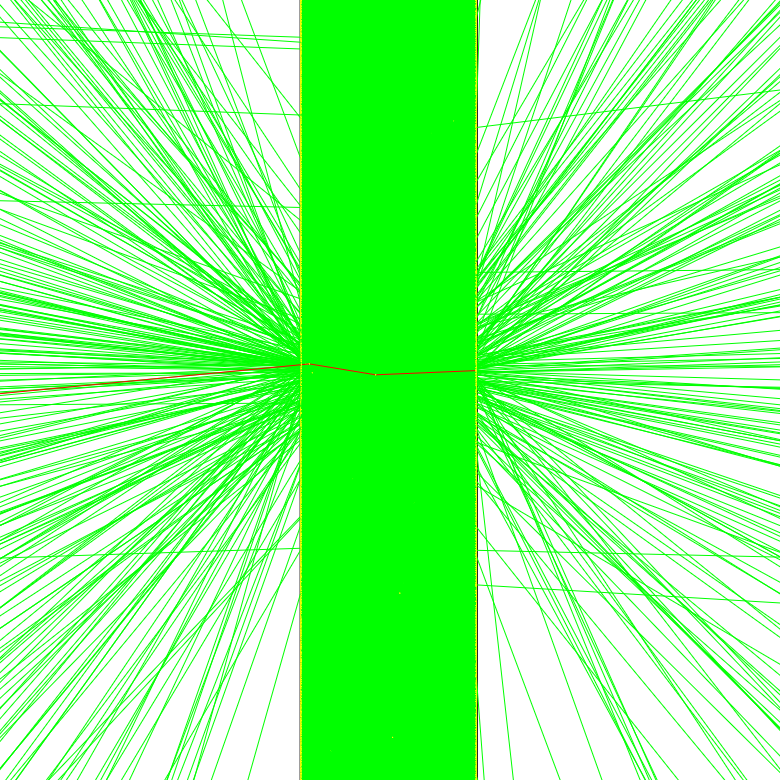
\includegraphics[width=0.9\linewidth]{Chapter4/Figs/Raster/lengthOnViewSliceElectron780Square.png}
  \captionsetup{width=.9\linewidth}
  \caption{Side on view.}
  \label{subFig:lengthOnViewSliceElectron780Square}
\end{subfigure}%
\begin{subfigure}{.5\textwidth}
  \centering
  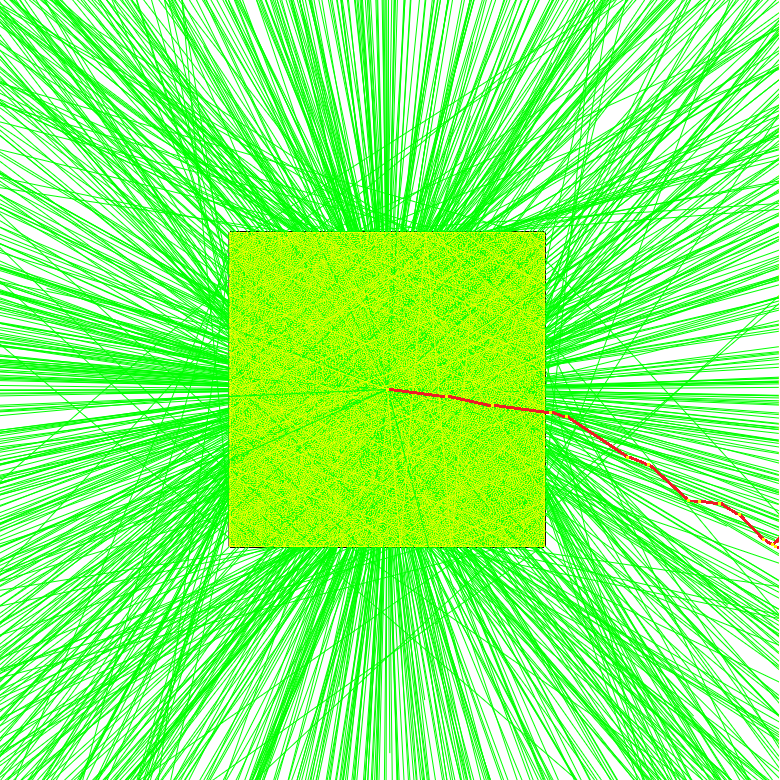
\includegraphics[width=0.9\linewidth]{Chapter4/Figs/Raster/sideOnViewSliceElectron780Square.png}
  \captionsetup{width=.9\linewidth}
  \caption{Length on view.}
  \label{subFig:sideOnViewSliceElectron780Square}
\end{subfigure}
\caption{A 1\,MeV e$^-$ particle (the red track) being simulated in a slice of plastic scintillator measuring 0.2\,m by 0.2\,m in (y,z) with 1\,mm thickness in x. Optical photons (the green tracks) are simulated to show how many are produced even over such a short distance at relatively low energies.}
\label{fig:lengthAndSideViewSliceElectron780Square}
\end{figure}

The ``slice'' model was used to determine the $S$ values for every particle in equation \ref{equ:Birks_formula}, once those had been obtained the $kB$ value of 0.0905 $\pm$ 0.015\,mm/MeV obtained from MINERvA was also used \cite{aliaga_2015}. By using the approximations $dL/dx \approx \Delta L / \Delta x$ and $dE/dx \approx \Delta E / \Delta x$ and using $\Delta L = L_{\textrm{end}} - L_{\textrm{start}} $ where in the simulation it is known that the light at the start of the step $L_{\textrm{start}} = 0$ and $L_{\textrm{end}}$ is the light at the end of each GEANT4 equation \ref{equ:light_produced} can be inferred. Using equation \ref{equ:light_produced} the light yield can now be calculated for the following particles were: $e^-$,$e^+$,$p$,$\bar{p}$,$\pi^+$,$\pi^-$,$\mu^-$,$\mu^+$,$\alpha$,$\bar{\alpha}$.

\begin{figure}[htbp]
\centering
\begin{subfigure}{.5\textwidth}
  \centering
  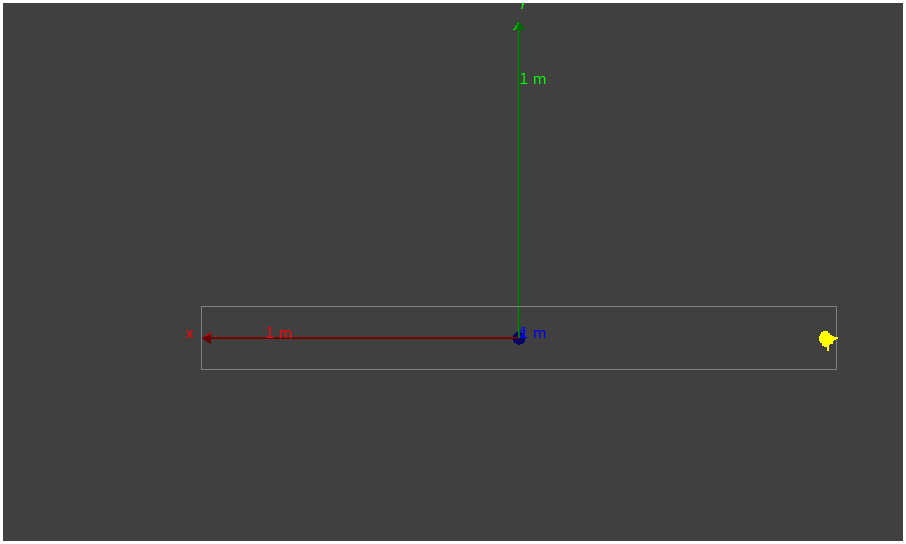
\includegraphics[width=\linewidth]{e-_10MeV_Length_on_view.png}
  \captionsetup{width=.9\linewidth}
  \caption{electrons side on view in ``slab''}
  \label{subFig:electron_side_slab}
\end{subfigure}%
\begin{subfigure}{.5\textwidth}
  \centering
  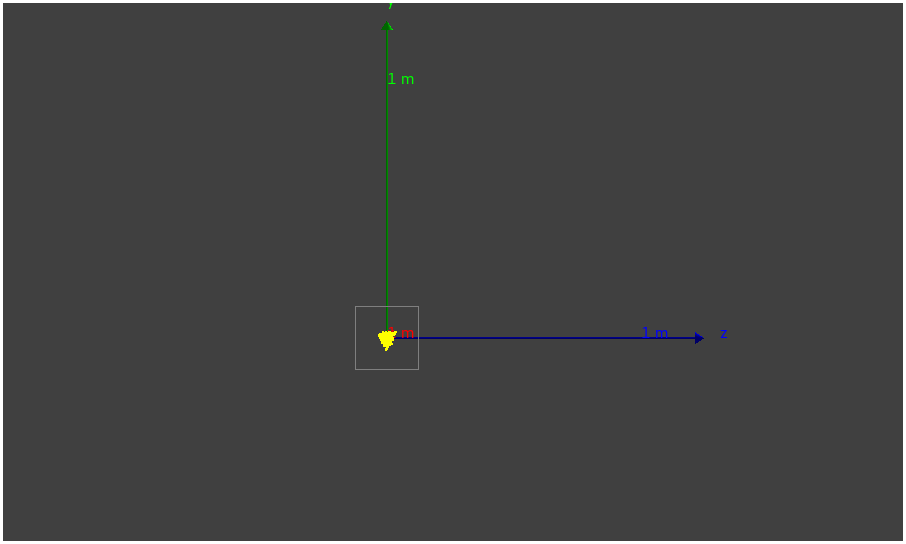
\includegraphics[width=\linewidth]{e-_10MeV_side_on_view.png}
  \captionsetup{width=.9\linewidth}
  \caption{electron length on view in ``slab''}
  \label{subFig:electron_length_slab}
\end{subfigure}
\caption{Electron side and length on view in ``slab'' of material, the electrons are not leaving the material. \hl{Change view to white background with black lines}.}
\label{fig:electrons_viewed_in_slab}
\end{figure}

\begin{equation}
L_{\textrm{end}}\approx \Delta x \left(\frac{S\frac{\Delta E}{\Delta x}}{1 + kB \frac{\Delta E}{\Delta x}}\right) 
\label{equ:light_produced}
\end{equation}
\\The approximations that Birk's law predicts for $p$,$\overline{p}$,$\pi^+$,$\pi^-$,$\mu^-$,$\mu^+$,$\alpha$,$\overline{\alpha}$ are very close to the model of light that GEANT4 predicts. The deviation from GEANT4 is at the worst at 100\,MeV where there is a deviation of $\sim$ $3\%$ in light output between GEANT4 and the Birks approximation of protons and anti-protons seen in figure \ref{fig:proton_aproton_light}, with \ref{subFig:proton_light} representing protons and \ref{subFig:aproton_light} representing anti-protons. In figure \ref{fig:proton_aproton_light} the Brik's approximation is a closer fit to the data than the simulated light fit which is a square function ($L = aE^2 + bE+ c$). A full table of S values can be seen in table \ref{tab:sValueTable}. Note how the positron S value is above the maximum photon limit of 1E5. 

\begin{table*}[htbp]
\centering
\begin{tabular}{lllll}  
\toprule
Particle       & kB [mm/MeV]        & S [photons/MeV] \\
\midrule
$\alpha$       & 0.0905 $\pm$ 0.015 & 9981.67 $\pm$ \hl{errors tbd}\\
$\bar{\alpha}$ & ....               & 9982.36 $\pm$ \hl{errors tbd}\\
$P$            & ....               & 9732.02 $\pm$ \hl{errors tbd}\\
$\bar{P}$      & ....               & 9788.46 $\pm$ \hl{errors tbd}\\
$\pi^+$        & ....               & 9702.75 $\pm$ \hl{errors tbd}\\
$\pi^-$        & ....               & 9728.48 $\pm$ \hl{errors tbd}\\
$\mu^-$        & ....               & 9987.57 $\pm$ \hl{errors tbd}\\
$\mu^+$        & ....               & 9970.17 $\pm$ \hl{errors tbd}\\
$e^-$          & ....               & 9549.41 $\pm$ \hl{errors tbd}\\
$e^+$          & ....               & 13003.5 $\pm$ \hl{errors tbd}\\
\bottomrule  
\end{tabular}
\caption{The kB and S values for each particle in the simulation found via the Birk's equation. The kB value is from MINERvA and is the sme for each particle. The maximum photon yield is 10000/MeV suggesting something is very wrong with the $e^+$ measurement. \hl{I need to redo this simulation stuff to get fits so I can get errors for S values}.}
\label{tab:sValueTable}
\end{table*}

\begin{figure}[htbp]
\centering
\begin{subfigure}{.5\textwidth}
  \centering
  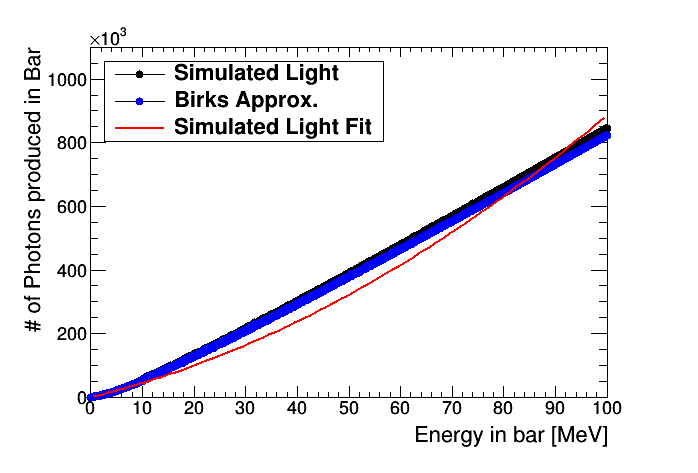
\includegraphics[width=\linewidth]{light_of_protons0-100mev.png}
  \captionsetup{width=.9\linewidth}
  \caption{Proton light produced by GEANT4 compared to the Birk's approximation of that light, the simulated light fit is the square function $L = aE^2 + bE+ c$ and is fit to the GEANT4 simulated light}
  \label{subFig:proton_light}
\end{subfigure}%
\begin{subfigure}{.5\textwidth}
  \centering
  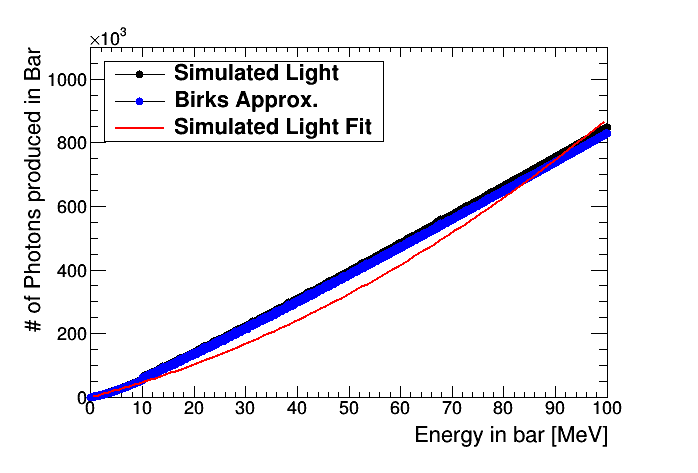
\includegraphics[width=\linewidth]{light_of_Aprotons0-100mev.png}
  \captionsetup{width=.9\linewidth}
  \caption{Anti-proton light produced by GEANT4 compared to the Birk's approximation of that light, the simulated light fit is the square function $L = aE^2 + bE+ c$ and is fit to the GEANT4 simulated light}
  \label{subFig:aproton_light}
\end{subfigure}
\caption{Proton and anti-proton light output compared to the birks approximation and a square fit to the light out put in GEANT4.}
\label{fig:proton_aproton_light}
\end{figure}

However the light yield for electrons and positrons seen in figure \ref{fig:electron_positron_light} varies more significantly. At 100\,MeV a variation of $\sim$ 15\,\% is seen in the electrons (figure \ref{subFig:electron_light}) and a variation and a variation of $\sim$ 20\,\% is seen in positrons (figure \ref{subFig:positron_light}). In figure \ref{fig:electron_positron_light} the simulated light which is a square function more accurately represents the GEANT4 light predictions. Figure \ref{fig:square_electron_positron_light} shows this approximation inputted instead. There is a slight variation between the simulated light fit and the square approximation seen in figures \ref{subFig:square_electron_light} (e$^-$) and \ref{subFig:square_positron_light} (e$^+$). This is because the simulated light fit fits to the whole light distribution whereas the light produced by the approximation in simulation is produced per GEANT4 step. Despite this, the square approximation for e$^-$ light ($L = 0.9347E^2 + 10340E - 0.1000$) had a variation of 0.7\,\% at 100\,MeV and the square approximation of the e$^+$ light ($L = 0.9716E^2 + 10350E -0.1000$) had a variation of 0.3\,\% at 100\,MeV. 
\begin{figure}[htbp]
\centering
\begin{subfigure}{.5\textwidth}
  \centering
  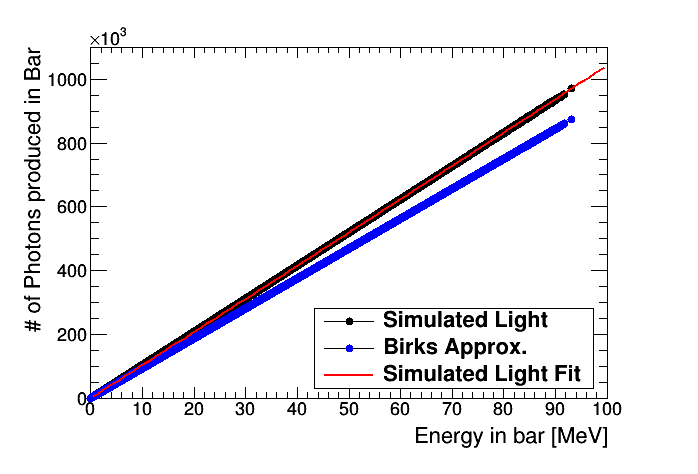
\includegraphics[width=\linewidth]{light_of_electrons0-100mev.png}
  \captionsetup{width=.9\linewidth}
  \caption{Electron light produced by GEANT4 compared to the Birks approximation of that light, the simulated light fit is the square funciton $L = aE^2 + bE+ c$ and is fit to the GEANT4 simulated light}
  \label{subFig:electron_light}
\end{subfigure}%
\begin{subfigure}{.5\textwidth}
  \centering
  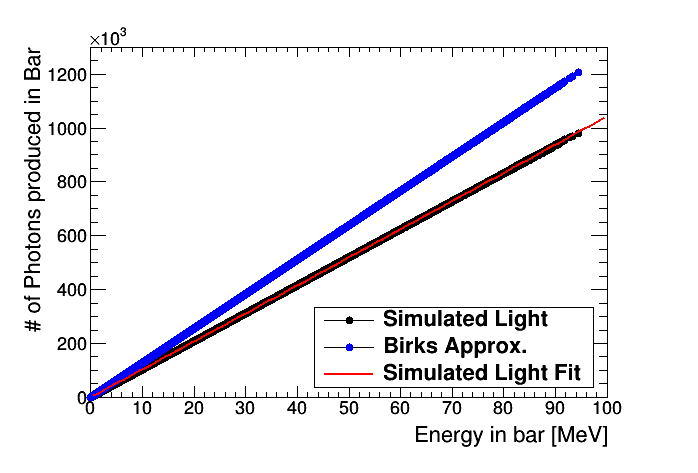
\includegraphics[width=\linewidth]{light_of_positrons0-100mev.png}
  \captionsetup{width=.9\linewidth}
  \caption{Positron light produced by GEANT4 compared to the Birks approximation of that light, the simulated light fit is the square funciton $L = aE^2 + bE+ c$ and is fit to the GEANT4 simulated light}
  \label{subFig:positron_light}
\end{subfigure}
\caption{Electron, Positron light output compared to the birks approximation and a square fit to the light out put in GEANT4}
\label{fig:electron_positron_light}
\end{figure}
\begin{figure}[htbp]
\centering
\begin{subfigure}{.5\textwidth}
  \centering
  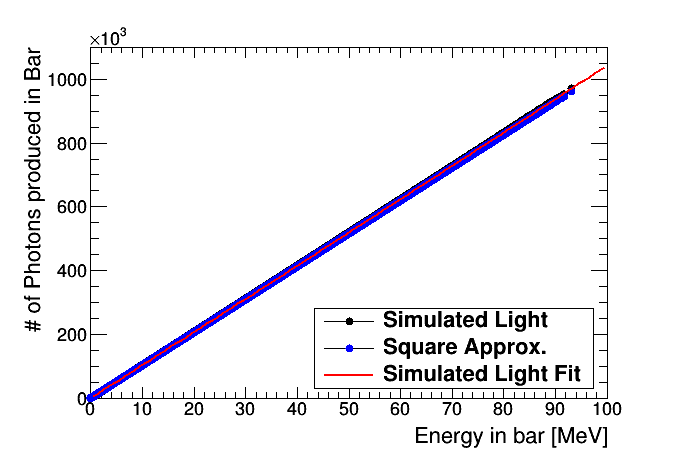
\includegraphics[width=\linewidth]{light_of_electronsLin0-100mev.png}
  \captionsetup{width=.9\linewidth}
  \caption{Electron light simulated by GEANT4 compared to the square approximation $L = aE^2 + bE+ c$ }
  \label{subFig:square_electron_light}
\end{subfigure}%
\begin{subfigure}{.5\textwidth}
  \centering
  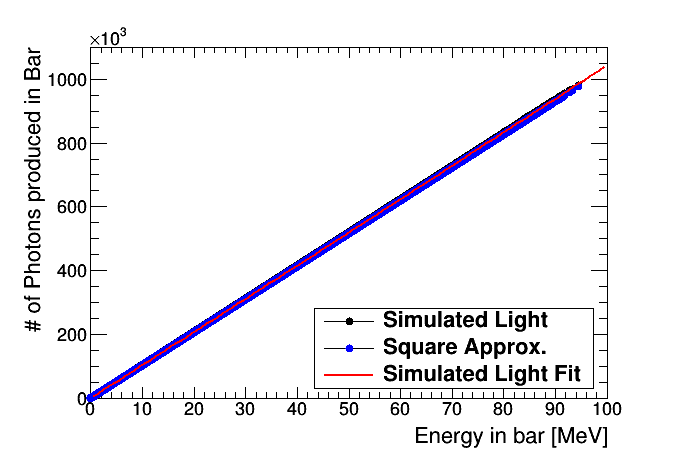
\includegraphics[width=\linewidth]{light_of_positronsLin0-100mev.png}
  \captionsetup{width=.9\linewidth}
  \caption{Positron light simulated by GEANT4 compared to the square approximation $L = aE^2 + bE+ c$}
  \label{subFig:square_positron_light}
\end{subfigure}
\caption{Electron and positron light output from simulation compared to a GEANT4 step square approximation}
\label{fig:square_electron_positron_light}
\end{figure}
\\\\The conversion of light into energy for electrons (figure \ref{subFig:square_electron_light}) is defined by equation \ref{equ:MeV_electron_equivalent_square}. The light of an electron is the highest amount of light per MeV that a particle can deposit this MeV electron equivalent (MeVee) is a special nomenclature used to describe the absolute light yield \cite{knoll_2010}. In equation \ref{equ:MeV_electron_equivalent_square} the squared term $ << $ the linear term, therefore the squared term is ignored for the purposes of light conversion, producing equation \ref{equ:MeV_electron_equivalent_linear}. By rearranging equation \ref{equ:MeV_electron_equivalent_linear} for energy production equation \ref{equ:MeV_electron_equivalent_light} is produced. The same is done for e$^+$ producing equation \ref{equ:MeV_postirtron_equivalent_light} . A small value of 0.1 is present in equations \ref{equ:MeV_electron_equivalent_linear}, \ref{equ:MeV_electron_equivalent_square}, \ref{equ:MeV_electron_equivalent_light}, \ref{equ:MeV_postirtron_equivalent_light} this is to prevent negative energy values being produced in equation \ref{equ:MeV_electron_equivalent_light}.  The reason the light yield is so different for e$^-$ and e$^+$ is due to the quenching effect being combined with the straggling effect. Range straggling is caused when particles have differing track lengths inside the scintillator thus depositing differing amounts of energy. These variable track lengths for e$^-$ and e$^+$ are due mostly to their small mass, for heavy charged particles such as protons or $\alpha$s the straggling amounts to a few percent of the mean range\cite{knoll_2010}. Hence e$^-$ and e$^+$ require a different light model to other charged particles.
\begin{equation}
L = 0.9347E^2 + 10340E - 0.1000
\label{equ:MeV_electron_equivalent_square}
\end{equation}
\begin{equation}
L = 10340E - 0.1000
\label{equ:MeV_electron_equivalent_linear}
\end{equation}
\begin{equation}
E = \frac{L +0.1000}{10340} 
\label{equ:MeV_electron_equivalent_light}
\end{equation}
\begin{equation}
E = \frac{L +0.1000}{10347.1}
\label{equ:MeV_postirtron_equivalent_light}
\end{equation}

\section{Loss of Deposited Energy due to Quenching}\label{sec:GEANT4Simulation_quenchingLoss}
Now the light has been suitably approximated from GEANT4 a quick investigation into the energy lost via quenching is required. The energy loss due to quenching varies greatly depending on the particle, it is a function of both energy and mass. By considering three example particles and their corresponding anti-particles the scale of the quenching in the VIDARR detector can be observed. The first particles to considered were be electrons. They are a common source of background and have a large charge to mass ratio when compared to other particles. The for electrons and positrons is very minimal which can be seen in figure \ref{fig:electron_positron_quenched_and_not}. This was simulated using a ``slab'' of material (figure \ref{fig:electrons_viewed_in_slab}) instead of using a bar or a full detector simulation. This was done to ensure that all of the energy was kept inside the plastic scintillator so that the full energy loss due to quenching could be measured. But in the case of e$^-$ and e$^+$ this is minimal. 

\begin{figure}[htbp]
\centering
\begin{subfigure}{.5\textwidth}
  \centering
  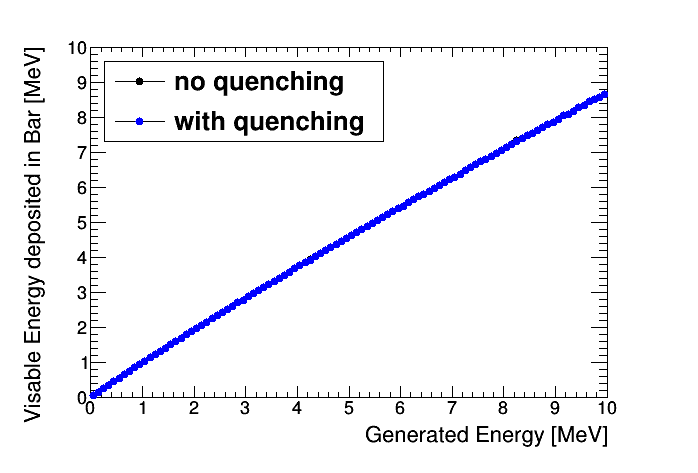
\includegraphics[width=\linewidth]{quench_eng_LinElectrons.png}
  \captionsetup{width=.9\linewidth}
  \caption{Visible electron energy deposition with and without quenching}
  \label{subFig:electron_quenched_and_not}
\end{subfigure}%
\begin{subfigure}{.5\textwidth}
  \centering
  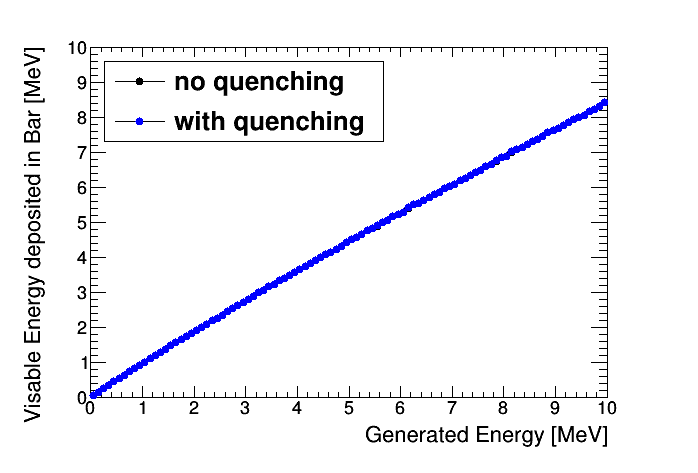
\includegraphics[width=\linewidth]{quench_eng_LinPositrons.png}
  \captionsetup{width=.9\linewidth}
  \caption{Visible positron energy deposition with and without quenching}
  \label{subFig:positron_quenched_and_not}
\end{subfigure}
\caption{Electrons and positrons visible energy with and without quenching in a ``slab'' of material (see figure \ref{fig:electrons_viewed_in_slab}).}
\label{fig:electron_positron_quenched_and_not}
\end{figure}

The effect of quenching on protons is much more significant than for electrons, the charge for protons is equal and opposite for electrons but the mass is $\sim$ 2000 times greater. This results in a large amount of energy no longer being deposited in the scintillator which can be seen in figure \ref{fig:proton_Apronton_quenched_and_not}. In figures \ref{subFig:proton_quenched_and_not} (protons) and \ref{subFig:Aproton_quenched_and_not} (anti-protons) the energy deposition is linear without quenching showing that for protons and anti-protons the effect of quenching is significant. For $\alpha$ particles the effect is even more significant $\alpha$ particles which are 4 times more massive than protons but have twice the charge. The loss due to quenching for protons varies from 90\,\% at a generated energy of 1\,MeV to 50\,\% at a generated energy of 10\,MeV (see figure \ref{fig:proton_Apronton_quenched_and_not}). But the effect for $\alpha$ particles is even more significant with almost none of the energy being visible below 1\,MeV and only 10\,\% of energy visible at 10\,MeV. By looking at figures \ref{fig:electron_positron_quenched_and_not}, \ref{fig:proton_Apronton_quenched_and_not}, and \ref{fig:alpha_Aalpha_quenched_and_not} it is easy to see the effect of quenching scaling with mass. This is the primary reason why simulating particles more massive than $\alpha$ particles is not done for VIDARR. Particles more massive than $\alpha$ particles will be quenched to such a point that they are unlikely to deposited a noticeable amount of energy in the detector's scintillator. 

\begin{figure}[htbp]
\centering
\begin{subfigure}{.5\textwidth}
  \centering
  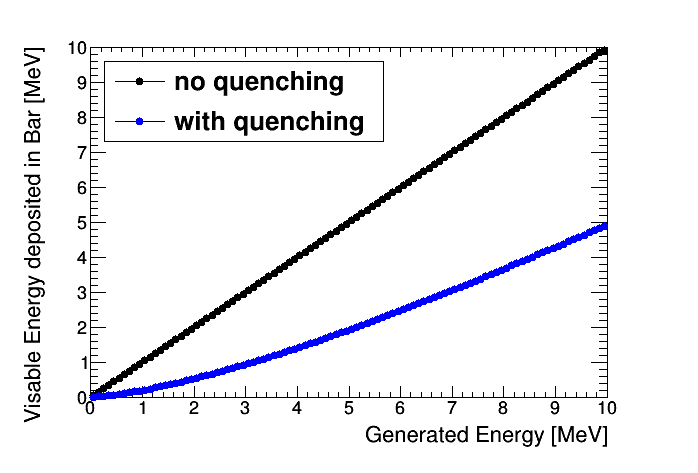
\includegraphics[width=\linewidth]{quench_eng_protons.png}
  \captionsetup{width=.9\linewidth}
  \caption{Visible proton energy deposition with and without quenching}
  \label{subFig:proton_quenched_and_not}
\end{subfigure}%
\begin{subfigure}{.5\textwidth}
  \centering
  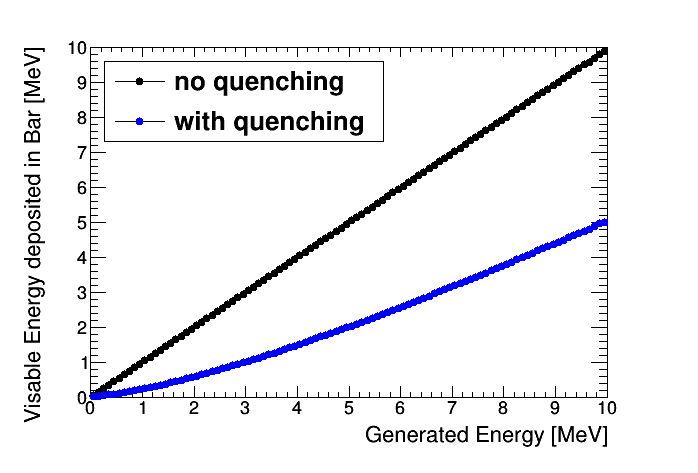
\includegraphics[width=\linewidth]{quench_eng_Aprotons.png}
  \captionsetup{width=.9\linewidth}
  \caption{Visible anti-proton energy deposition with and without quenching}
  \label{subFig:Aproton_quenched_and_not}
\end{subfigure}
\caption{protons and anti-protons visible energy with and without quenching in a ``slab'' of material (see figure \ref{fig:electrons_viewed_in_slab})}
\label{fig:proton_Apronton_quenched_and_not}
\end{figure}

\begin{figure}[htbp]
\centering
\begin{subfigure}{.5\textwidth}
  \centering
  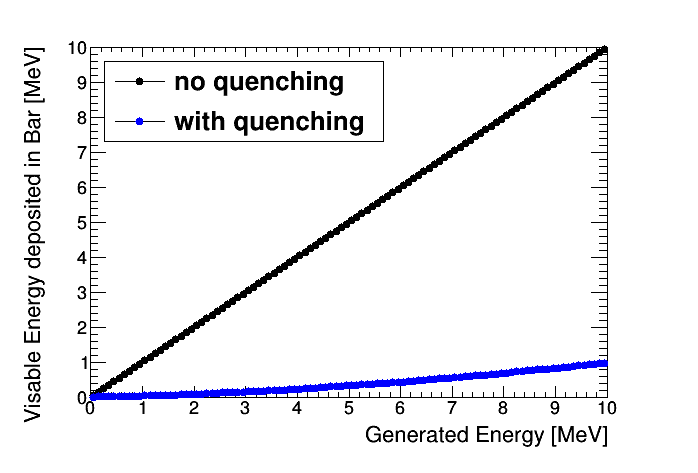
\includegraphics[width=\linewidth]{quench_eng_Alpha.png}
  \captionsetup{width=.9\linewidth}
  \caption{Visible $\alpha$ particle energy deposition with and without quenching}
  \label{subFig:alpha_quenched_and_not}
\end{subfigure}%
\begin{subfigure}{.5\textwidth}
  \centering
  \includegraphics[width=\linewidth]{quench_eng_AAlpha.png}
  \captionsetup{width=.9\linewidth}
  \caption{Visible $\bar{\alpha}$ particle energy deposition with and without quenching}
  \label{subFig:Aalpha_quenched_and_not}
\end{subfigure}
\caption{$\alpha$ and $\bar{\alpha}$ particles visible energy with and without quenching in a ``slab'' of material (see figure \ref{fig:electrons_viewed_in_slab}).}
\label{fig:alpha_Aalpha_quenched_and_not}
\end{figure}

\section{Counting Statistics} \label{sec:GEANT4Simulation_countingStats}
When a particle passes through the scintillating plastic it produces photons as it interacts. These photons then travel through the bar until they meet the WLS fibres. The photons then travel down the WLS fibres until they encounter the MPPC  this signal is then amplified by the MPPC producing a signal of 4.2\,mV which is equivalent for one photon see figure \ref{fig:pureDarkNoise} which is called a photo-electron equivalent (PE). So for n number of photo-electron equivalents there will be a Poisson distribution (equation \ref{equ:possionProb}) associated with it due to counting statistics. A Poisson approximation is suitable because there is a small probability of a given outcome in this case. For this distribution $pn = \overline{x}$ where $\overline{x}$ is the expectation value, substituting this into equation \ref{equ:possionProb} we get equation \ref{equ:possionExpectation} \cite{knoll_2010}.
\begin{equation}
P(x) = \frac{(pn)^x e^{-pn}}{x!}  
\label{equ:possionProb}
\end{equation}

\begin{equation}
P(x) = \frac{(\overline{x})^x e^{-\overline{x}}}{x!}  
\label{equ:possionExpectation}
\end{equation}

Further the variance of this model can be explained using equation  \ref{equ:possionVar} which also gives $\sigma^2 = \overline{x}$ giving a standard deviation of $\sigma = \sqrt{\overline{x}}$ \cite{knoll_2010}. This definition of the standard deviation is also true for the Gaussian distribution. The Gaussian distribution using this standard deviation can be seen in equation \ref{equ:guassianExpectation}. When n is high enough the Poisson distribution will approximate to a Gaussian distribution this is useful when simulating light counting statistics because a Gaussian distribution is much less computationally intensive as there is no factorial. The point where Gaussian is used instead of Poisson in the simulation is at a value of 10 photons seen in figure \ref{fig:CoutingStats10}. At an expectation value of 10 photons 99.9\,\% of events produce have $>$ 2 photons in the Poisson distribution (see figure \ref{fig:CoutingStats10}). This is a useful limit to switch distributions as it ensures that the low values of PE correctly modelled by the Poisson distribution are minimal. 

\begin{equation}
\sigma ^2 \equiv \sum_{x=0}^{n} (x-\overline{x})^2 P(x) = pn = \overline{x} 
\label{equ:possionVar}
\end{equation}

\begin{equation}
P(x) = \frac{1}{\sigma \sqrt[]{2 \pi}} \exp \left(-\frac{1}{2}\left(\frac{x-\overline{x}}{\sigma}\right)^{2}\right)
\label{equ:guassianExpectation}
\end{equation}

\begin{figure}[htbp]
 \centering
 \includegraphics[width=0.8\linewidth]{countingStats10.png}
 \captionof{figure}{Counting statistics for Poisson and normal distribution for an expectation value of 10 photons the normal distribution is used when the expectation value is $\geq$ 10 photons 
 to save on computational load. \hl{plot could do with some prettying...}} 
 \label{fig:CoutingStats10}
\end{figure}

\section{Simulated Results With Physical and Electronic Effects}\label{sec:GEANT4Simulation_resultsPhysicalElectronics}
The impact of physical and electronic effects on simulated data is quite significant especially for heavier particles such as protons and $\alpha$s. The heaviest particle we expect to see in statistically significant quantities is the $\alpha$. In order to show the maximum difference between generated and a more realistic simulation generated $\alpha$ particles are used for this section. 
\\\\If these effects ignored in the simulation then the results look nonphysical. In figure \ref{fig:alpha_summed_vs_truth} the summed energy inside the detector is equal to the truth energy in most cases. This is because the additional effects are being ignored and only the energy deposited in the scintillator is being reconstructed. The only events which do not have all the energy summed in the detector are those which were generated near the edges of the bar, these events are absorbed by the TiO$_2$ coating and so deposit less energy in the detector. The modelling of quenching (see section \ref{sec:GEANT4Simulation_MonteCarloBirksLaw}) and attenuation (see figure \ref{fig:attenuationPlot}) therefore cause a large decrease in the summed energy inside the detector seen in figure \ref{fig:alphaVisVsTruthZoom}. Figure \ref{fig:alphaVisVsTruthZoom} is an idealistic representation of what $\alpha$ particles would look like in a VIDARR detector with perfect electronics. I.e no losses or distortions.

\begin{figure}[htbp]
 \centering
 \includegraphics[width=0.7\linewidth]{truth_vs_summed_alpha.png}
 \captionof{figure}{The energy deposited in a simulated detector by $\alpha$ particles without physical and electronic effects taken into account, this is the maximum possible energy that can be deposited.} 
 \label{fig:alpha_summed_vs_truth}
\end{figure}
\begin{figure}[htbp]
 \centering
 \includegraphics[width=0.7\linewidth]{Chapter4/Figs/Raster/truth_vs_visSummed_alpha_zoom.png}
 \captionof{figure}{The energy deposited in a simulated detector by $\alpha$ particles with only the physical effects of quenching and attenuation taken into account. The detector effects of dark noise and counting statistics are not taken into account} 
 \label{fig:alphaVisVsTruthZoom}
\end{figure}


Finally the effects caused by the electronics (figure \ref{fig:fitting_of_non_peak_dark_noise}) and the counting statistics (figure \ref{fig:CoutingStats10}) gives the simulated distribution a more realistic shape. The results for this can be seen in figure \ref{fig:alphaRecoVsTruthZoom}. With the data driven effects taken into account the simulation should give a more realistic result. Unfortunately due to the outbreak of Covid-19 the detector construction was delayed and so the accuracy of the simulation cannot be bench marked against detector data. 

\begin{figure}[htbp]
 \centering
 \includegraphics[width=0.7\linewidth]{Chapter4/Figs/Raster/truth_vs_recoSummed_alpha_zoom.png}
 \captionof{figure}{The energy deposited in a simulated detector by $\alpha$ particles with physical effects of quenching and attenuation taken into account as well as the detector effects of dark noise and counting statistics.} 
 \label{fig:alphaRecoVsTruthZoom}
\end{figure}

\section{Modelling Gadolinium}\label{sec:GEANT4Simulation_modellingGadolinium}
The Gadolinium cascade is difficult to measure and accurately simulate for for two main reasons. Firstly the Gd isotopes which have a high neutron capture cross-section are isotopes $^155$Gd and $^157$Gd \cite{molnar_2004}. Both of these nuclei are large therefore it is difficult to accurately model the individual interactions between each of the individual nucleons. There is no agreed upon model at present for the neutron absorption onto Gadolinium and the subsequent 8\,MeV $\gamma$ cascade. The second issue is that the high energy $\gamma$ rays emitted by the cascade are very difficult to contain. Therefore, getting accurate measurements and energy efficiencies for the cascade is also very difficult. These two problems compound one another. It is difficult to measure the cascade so it is difficult to model thus making it difficult to know what energies are expected from the Gd nucleus. Further issues are caused by the highly penetrative nature of high energy $\gamma$ rays thus making efficiency estimates even less accurate \cite{molnar_2004}. Gadolinium is used because of its high efficiency (10$\%$ - 40$\%$) compared to other neutron capturing materials such as $^6$Li which only has about $1\%$ \cite{Abdushukurov_2010}. The 8\,MeV $\gamma$ cascade post neutron absorption is the trigger signal for the VIDARR detector. After the cascade has been triggered the detector looks backwards in time to determine the e$^+$ cluster.
\\\\Gadolinium has two models in Geant 4 the photon evaporation model seen in \ref{subFig:differentGEANT4Models_photonEvaporationGd} and the final state model seen in  \ref{subFig:differentGEANT4Models_finalStateGd}. These two models have different strengths and weaknesses the photon evaporation model conserves energy by ``boiling off'' the known decay energies of Gadolinium until there is no more energy left to disperse. This approach attempts to match the multiplicity of the gadolinium cascade but in so doing the high energy $\gamma$ rays that are the most indicative of the gadolinium cascade are not present. The other model in Geant 4 is the final state model which tries to match the spectrum of measured energy rays. However, by using this approach the conservation of energy is violated. As the sum of the individual $\gamma$ rays exceeds the initial generated energy. Of the two models the final state is preferred in the case of IBD. This is because the high energy $\gamma$ rays that distinguish the gadolinium cascade from background are present in the final state model and not the photon evaporation model.

\begin{figure}[htbp]
\centering
\begin{subfigure}{.5\textwidth}
  \centering
  \includegraphics[width=\linewidth]{Chapter4/Figs/Raster/gadolinium/photonEvaporationGd.png}
  \captionsetup{width=.9\linewidth}
  \caption{GEANT4 photon evaporation model.}
  \label{subFig:differentGEANT4Models_photonEvaporationGd}
\end{subfigure}%
\begin{subfigure}{.5\textwidth}
  \centering
  \includegraphics[width=\linewidth]{Chapter4/Figs/Raster/gadolinium/FinalStateGd.png}
  \captionsetup{width=.9\linewidth}
  \caption{GEANT4 final state model.}
  \label{subFig:differentGEANT4Models_finalStateGd}
\end{subfigure}
\caption{Individual $\gamma$ rays for two different models for gadolinium cascade in GEANT4. The photon evaporation model which conserves energy but does not produce high energy $\gamma$ rays (figure \ref{subFig:differentGEANT4Models_photonEvaporationGd}). The final state model produces high energy $\gamma$ rays but breaks the conservation of energy to do so (figure \ref{subFig:differentGEANT4Models_finalStateGd}). Both plots from \cite{YuChen_2015}.}
\label{fig:differentGEANT4Models}
\end{figure}

%I'm not sure how useful this plot is... Natural Gadolinium is mentioned later with more context
% \begin{figure}[htbp]
%  \centering
%  \includegraphics[width=0.7\linewidth]{Chapter4/Figs/Raster/gadolinium/naturalGd.png}
%  \captionof{figure}{Natural Gadolinium gamma spectra from \cite{molnar_2004}} 
%  \label{fig:naturalGd.png}
% \end{figure}

However, whilst the final state model is preferable to the photon evaporation model there is another alternative from the DANCE collaboration which produced a dicebox model of $^{157}$Gd \cite{Chyzh_2011}. DANCE is a $\gamma$ calorimeter consisting of 160 BaF$_2$ scintillation detectors. The multiplicities of the cascade from the dicebox are counted as the number of clusters that are observed rather than the number of crystals that fire in order to give a more accurate measurement of multiplicity due to the high noise rate observed in the detectors below 3\,MeV \cite{Chyzh_2011}. The shape of the spectrum at low sum energies (below about 3 MeV) is strongly influenced by the background from natural $\beta$ activity in the BaF2 crystals, especially for low multiplicities \cite{Chyzh_2011}. Measuring the number of clusters should reduce the errors for low multiplicty according to DANCE \cite{Chyzh_2011}. The breakdown for the multiplicity cascade can be seen in figure \ref{fig:gadoliniumMultipliciesBreakdownCascade} where both the $\gamma$ and e$^-$ multiplicities are shown. Most of the multiplicities are driven by the $\gamma$ rays but the some e$^-$s are produced unlike the models in GEANT4. 

\begin{figure}[htbp]
 \centering
 \includegraphics[width=0.7\linewidth]{Chapter4/Figs/Raster/gadolinium/gadoliniumMultipliciesBreakdownCascade.png}
 \captionof{figure}{Multiplicities from the DANCE dicebox based on the DANCE experimental data for $^{157}$Gd \cite{Chyzh_2011}. } 
 \label{fig:gadoliniumMultipliciesBreakdownCascade}
\end{figure}

The breakdown for all the energies for the DANCE dicebox is shown in figure \ref{fig:gadoliniumEnergiesCascade} where most of the energies produced are $\gamma$ rays. The dominance of the $\gamma$ rays is not surprising when comparing the dicebox to the photon evaporation and final state models in GEANT4 (figure \ref{fig:differentGEANT4Models}). The generated energies for all of the particles can be seen in figure \ref{fig:energyOfCascadeOfCascadeGd} these energies are what is put into the GEANT4 simulation as well as the type of particle. The WATCHMAN collaboration created a method to integrate the DANCE dicebox into GEANT4 by cancelling the 8\,MeV $\gamma$ cascade and forcing new secondary production via the DANCE dicebox. This implementation was copied by the VIDARR collaboration. In figure \ref{fig:energyOfCascadeOfCascadeGd} high energy $\gamma$ rays are visible unlike in the photon evaporation model (figure \ref{subFig:differentGEANT4Models_photonEvaporationGd}). However, the DANCE dicebox model also conserves energy, the total amount of energy can be seen in figure  \ref{fig:conservationOfCascadeGd}. For the DANCE dicebox the total generated energy matches the summed energy of the particles produced in contrast to the final state model. 

\begin{figure}[htbp]
 \centering
 \includegraphics[width=0.7\linewidth]{Chapter4/Figs/Raster/gadolinium/gadoliniumEnergiesCascade.png}
 \captionof{figure}{Energies from the DANCE dicebox based on the DANCE experimental data for $^{157}$Gd \cite{Chyzh_2011}. } 
 \label{fig:gadoliniumEnergiesCascade}
\end{figure}

% \begin{figure}[htbp]
%  \centering
%  \includegraphics[width=0.7\linewidth]{Chapter4/Figs/Raster/gadolinium/pe_vs_fs_models_summed.png}
%  \captionof{figure}{blah.} 
%  \label{fig:pe_vs_fs_models_summed}
% \end{figure}

\begin{figure}[htbp]
 \centering
 \includegraphics[width=0.7\linewidth]{Chapter4/Figs/Raster/gadolinium/energyOfCascadeOfCascadeGd.png}
 \captionof{figure}{Energy of all particles from the $^{157}$Gd dicebox based on the DANCE experiment \cite{Chyzh_2011} which is then worked into GEANT4 using an implementation created by the WATCHMAN collaboration which was then copied by the VIDARR collaboration.} 
 \label{fig:energyOfCascadeOfCascadeGd}
\end{figure}

\begin{figure}[htbp]
 \centering
 \includegraphics[width=0.7\linewidth]{Chapter4/Figs/Raster/gadolinium/conservationOfCascadeGd.png}
 \captionof{figure}{The summed energy for the Dicebox gadolinium $\gamma$ cascade. There is no violation of the conservation of energy 8\,MeV energy is generated and 8\,MeV is observed by the simulation.} 
 \label{fig:conservationOfCascadeGd}
\end{figure}

The photon evaporation model and final state model were overlapped with the measured spectrum from natural gadolinium as well as $^{155}$Gd,$^{157}$Gd in figure \ref{fig:comparisonGd}. The high energy $\gamma$ rays observed in the natural and specific isotopes of Gd are present in the final state model which reads from the data base ENDF and tries to replicate the final state of the neutron \cite{koiTatsumi_2006}. With the final state model events in the low energy tail break Q-value (conservation of energy) \cite{YuChen_2015}. When DANCE/WATCHMENT dicebox overlaid on top of the photon evaporation model and the final state model as shown in figure  \ref{fig:comparisonAndDiceBoxGd} the dicebox seems very similar to the photon evaporation model but extends further producing more higher energy $\gamma$ rays. The dicebox shown in figure \ref{fig:comparisonAndDiceBoxGd} only represents $^{157}$Gd. The DANCE dicebox was based on data measured from a sample that was  99.7\,\% $^{157}$Gd \cite{Chyzh_2011}. 

\begin{figure}[htbp]
 \centering
 \includegraphics[width=0.7\linewidth]{Chapter4/Figs/Raster/gadolinium/comparisonGd.png}
 \captionof{figure}{How the photon evaporation and final state models in GEANT 4 compare to the measured spectra for natural gadolinium and Gd 155,157. High energy $\gamma$s are only present in the final state model.  * \cite{kandlakunta_2012} ** \cite{bollinger_1970} from \cite{YuChen_2015}.} 
 \label{fig:comparisonGd}
\end{figure}

\begin{figure}[htbp]
 \centering
 \includegraphics[width=0.7\linewidth]{Chapter4/Figs/Raster/gadolinium/comparisonAndDiceBoxGd.png}
 \captionof{figure}{Figure \ref{fig:comparisonGd} \cite{YuChen_2015} but with the Dicebox individual $\gamma$ rays for $^{157}$Gd from figure \ref{fig:energyOfCascadeOfCascadeGd} overlaid on top. The Dicebox has similar low energy $\gamma$ rays to the photon evaporation model but has more high energy $\gamma$ rays as would be expected of the Gd cascade. * \cite{kandlakunta_2012} ** \cite{bollinger_1970}.}
 \label{fig:comparisonAndDiceBoxGd}
\end{figure}

The energies of the $\gamma$ rays produced by the simulation are shown in figure \ref{fig:gdCascadeVsAllGammas}. The Gd Cascade is from a simulation of natural Gadolinium which uses the DANCE/WATCHMAN dicebox when $^{157}$Gd captures a neutron and uses the final state model when other isotopes of Gd capture a neutron. In figure \ref{fig:gdCascadeVsAllGammas} the majority of the $\gamma$ rays produced are from the $^{157}$Gd dicebox final state model hybrid. However, there is also a significant peak caused by the hydrogen neutron capture. The effect of adding the dicebox to the final state model can be seen in figure \ref{fig:TotalGeneratedEnergyOfCascadeFinalStateDicebox}. Compared to the final state model the peaks in the dicebox final state hybrid are much more pronounced with more energy being produced overall. The focus on the high energy $\gamma$ rays also means that more energy is deposited in the scintillator as well (figure \ref{fig:finalStateAndDiceBoxBarsDepositedEnergy}). This is very useful for the VIDARR simulation, not only is the dicebox-final state hybrid more realistic than the pure final state model it also shows that the trigger signal for the VIDARR detector is even more unique than expected. Not only depositing more energy in the scintillator than would be expected from the pure final state model (figure \ref{fig:finalStateAndDiceBoxBarsDepositedEnergy}) but also hits more bars as seen in figure \ref{fig:numberOfBarsHitCascadeFinalStateDicebox}. This is especially useful for separating out the trigger signal from the noise as will be shown in section \ref{sec:MachineLearningTrigger}.

\begin{figure}[htbp]
 \centering
 \includegraphics[width=0.7\linewidth]{Chapter4/Figs/Raster/gadolinium/gdCascadeVsAllGammas.png}
 \captionof{figure}{The individual $\gamma$ rays seen in the simulated VIDARR detector from generated neutrons with 0.025\,eV kinetic energy. The majority of the distribution is dominated by gadolinium cascade but a small peak is caused by the hydrogen absorption of the neutron.} 
 \label{fig:gdCascadeVsAllGammas}
\end{figure}

\begin{figure}[htbp]
 \centering
 \includegraphics[width=0.7\linewidth]{Chapter4/Figs/Raster/finalStateAndDiceBoxBarsGeneratedEnergy.png}
 \captionof{figure}{Total generated energy of the cascade the dicebox based on the DANCE detector data \cite{Chyzh_2011}.}
 \label{fig:TotalGeneratedEnergyOfCascadeFinalStateDicebox}
\end{figure}

\begin{figure}[htbp]
 \centering
 \includegraphics[width=0.7\linewidth]{Chapter4/Figs/Raster/finalStateAndDiceBoxBarsDepositedEnergy.png}
 \captionof{figure}{The total energy deposited in the simulated VIDARR detector. Slightly more energy is deposited by the final state + Dicebox model. (0th bin for Final state No $^{157}$Gd goes up to 80000)} 
 \label{fig:finalStateAndDiceBoxBarsDepositedEnergy}
\end{figure}

\begin{figure}[htbp]
 \centering
 \includegraphics[width=0.7\linewidth]{Chapter4/Figs/Raster/finalStateAndDiceBoxBarsHit.png}
 \captionof{figure}{The number of bars hit in the simulated VIDARR detector for different models. The final state model with the dicebox $^{157}$Gd was chosen and hits slightly more bars.} 
 \label{fig:numberOfBarsHitCascadeFinalStateDicebox}
\end{figure} 
 
\section{Machine Learning Neutron Trigger}\label{sec:MachineLearningTrigger}
Using simulated data it is possible to test weather a machine learning trigger would be advantageous to the analysis. The machine learning technique considered the most appropriate was the Support Vector Machine (SVM) \cite{Boser92atraining} \cite{cortes1995support}. SVMs were compared to several other simple techniques typically used in physics namely a decision tree and k nearest neighbours (see figure \ref{fig:sklearnReleventExamples}). As seen in figure \ref{fig:sklearnReleventExamples} the SVM linearly or with a kernel. The radial basis function (RBF) kernel is one of the most common. In figure \ref{fig:sklearnReleventExamples} the generalised boundaries, high accuracy, and well defined projection space seen in the RBF SVM makes it the clear standout. The SVM utalises the RBF kernal via the kernel trick since at least 1992 \cite{Boser92atraining}. 
\\\\SVMs work by finding the best separating hyperplane between two opposing data sets. In figure \ref{fig:svmBoser92LinearSVM} the best separating hyperplane is calculated for a simple data set. The SVM works by finding the maximum distance between each data set and creating an n dimensional line the ``hyperplane'' to separate the data. In order to separate non linear data the kernel trick is used which figure \ref{fig:svmBoser92KernelSVM} shows. Figure \ref{fig:svmBoser92KernelSVM} also shows how two different kernel achieve the same result. How the decision surface is manipulated to separate data sets is shown in figure \ref{fig:kernelRBF_fromWeB}. As figure \ref{fig:kernelRBF_fromWeB} shows the kernel transforms the data set so it becomes linearly separable for the SVM. A further test of the SVMS's capabilities is done in figure \ref{fig:svmExp_GausseExamples} which tests the separation of multiple Gaussian data sets from 2D exponential noise. This is as complex ass trigger data could reasonably be expected to be. This means that the SVM should be suitable for separating neutron trigger data. 
\\\\An SVM is also convexly optimised which means the solutions are easier to solve for as there is only one global minimum \cite{cortes1995support}. This feature allows SVMs to train on sparse data sets with low statistics. SVMs are fast to train on small data sets but as data sets grow larger the squared nature of the SVM solution increases training times dramatically \cite{cortes1995support}. This means that for data with many dimensions and many statistics training times and memory usage can be very high to the point of being unusable \cite{cortes1995support}. Data must also be completely labelled and optimisation for training whilst possible through sequential minimal optimisation is somewhat limited \cite{platt1998sequential}. These drawbacks are not a significant issue for the trigger data but they should be bared in mind for more complex cases such as image recognition.
 
\begin{figure}[htbp]
\centering
\includegraphics[width=\linewidth]{Chapter4/Figs/Raster/svmLinAndRbf/sklearnReleventExamples.png}
\captionof{figure}{Some example classifiers taken from scikit-learn that show how different techniques draw boundaries and how confident they are in those boundaries. Decision trees and k nearest neighbours are common simplistic classifiers used in physics but the boundaries they produce are often susceptible to over-training. The linear SVM is generalised but is quite limited in its utility. The SVM with the RBF kernel consistently draws the most accurate boundaries and they are well generalised. The accuracy of each technique is shown in the bottom right of each plot. From \cite{scikit-learn}.} 
\label{fig:sklearnReleventExamples}
\end{figure}

\begin{figure}[htbp]
\centering
\includegraphics[width=\linewidth]{Chapter4/Figs/Raster/svmLinAndRbf/svmBoser92LinearSVM.png}
\captionof{figure}{An example of a how a support vector machine (SVM) separates two different distributions that are linearly separable. The maths behind the classifier finds the best separating line/hyper-plane between two distributions. From \cite{Boser92atraining}.} 
\label{fig:svmBoser92LinearSVM}
\end{figure}

\begin{figure}[htbp]
\centering
\includegraphics[width=\linewidth]{Chapter4/Figs/Raster/svmLinAndRbf/svmBoser92KernelSVM.png}
\captionof{figure}{How a support vector machine (SVM) operates with a kernel being applied using a squared polynomial kernel on the left and a radial basis function (RBF) on the right . By using the ``kernel trick'' it is possible to separate non-linear data. From \cite{Boser92atraining}.} 
\label{fig:svmBoser92KernelSVM}
\end{figure}

\begin{figure}[htbp]
\centering
\includegraphics[width=\linewidth]{Chapter4/Figs/Raster/svmLinAndRbf/kernelRBF_fromWeB.png}
\captionof{figure}{An online example that shows how the kernel trick is used to make non-linear data linearly separable by transforming it through a kernel. From \cite{kernelTrickWeb}.} 
\label{fig:kernelRBF_fromWeB}
\end{figure}

\begin{figure}[htbp]
\centering
\begin{subfigure}{.5\textwidth}
  \centering
  \includegraphics[width=\linewidth]{Chapter4/Figs/Raster/svmLinAndRbf/svmExp_2GaussExample.png}
  \captionsetup{width=.9\linewidth}
  \caption{How LIBSVM draws boundaries around complex signal and noise data sets with an RBF kernel. Support vectors highlighted in orange.}
  \label{subFig:svmExp_2GausseExample}
\end{subfigure}%
\begin{subfigure}{.5\textwidth}
  \centering
  \includegraphics[width=\linewidth]{Chapter4/Figs/Raster/svmLinAndRbf/exp_2NysGaussExample.png}
  \captionsetup{width=.9\linewidth}
  \caption{How LIBLINEAR draws boundaries around complex signal and noise sets with a Nystrom approximation of the RBF kernel with a sampling of 100.}
  \label{subFig:exp_2NysGaussExample}
\end{subfigure}
\caption{SVM examples showing how to separate data sets with two Gaussian signals (blue) from exponential noise (red). For both an RBF kernel was used with c = 1e4 and $\gamma$ = 1. \hl{Axes need updating so the text is clearer}.}
\label{fig:svmExp_GausseExamples}
\end{figure}

Figures \ref{fig:sklearnReleventExamples} \ref{fig:svmBoser92LinearSVM} \ref{fig:svmBoser92KernelSVM} \ref{fig:kernelRBF_fromWeB} \ref{fig:svmExp_GausseExamples} are sufficient reason to believe that an SVM with an RBF kernel should be a suitable classifier for separating trigger data which only has four dimensions. The four dimensions that need to be optimised are: the summed energy above a threshold of 1.5\,PE (0.06\,MeV), summed energy above a threshold of 12.5\,PE (0.5\,MeV), Numbers of bars hit above a threshold of 1.5\,PE (0.06\,MeV), Numbers of bars hit above threshold 12.5\,PE (0.5\,MeV). The libraries used were LIBSVM and LIBLINEAR both of which are highly provident and often cited as the reason for the SVMs gain in popularity \cite{chang2011libsvm} \cite{fan2008liblinear} \cite{murty2016support}. The wrapper in sci-kit learn was the preferred method due to its ease of use and its convenient application of the Nystrom approximation \cite{williams2001using} of the kernel. The Nystroem approximation is useful as the amount of computation required for a complete kernel SVMs scales $\sim$ O (n$^3$) where n is the number of training examples \cite{williams2001using}. By using a sample of size m to compute an approximation of the kernel the amount of computation required scales $\sim$ O (m$^2$n) instead \cite{williams2001using}. This approach will work even when m $\ll$ n \cite{williams2001using}. The example data shown in \ref{fig:svmExp_GausseExamples} shows how LIBLINEAR when combined with with an RBF Nystroem approximated kernel performs in comparison to LIBSVM with a complete RBF kernel the boundaries are very similar. From this point the LIBLINEAR library and the Nystroem approximation will be used to speed up training and to prevent memory overflow which can happen when the SVM isn't converging and when large data sets are used. The simulated data set has 1 million neutron signal events and 4 million background events.
\\\\Kernel SVMs have two factors that can be tweaked to give more accurate results. The soft margin C higher values of C correspond to a lower amount of signal and noise overlap and vice versa \cite{cortes1995support}. Typically C can vary from 10$^{-6}$ to 10$^6$ but can be even higher or even lower. The other factor is $\gamma$ and is part of the RBF kernel shown in equation \ref{equ:RbfKernelFunc} and is taken from \cite{Boser92atraining}. The value for $\gamma$ must be $>$ 0. For an example of what non linear data looks like when searching for suitable C and $\gamma$ values figure \ref{fig:GammaCGridSearchExp2Gauss} was produced which shows how the values for figure \ref{subFig:exp_2NysGaussExample} where chosen. A higher value of $\gamma$ corresponds to higher non-linearity. With this information we can see that there is some overlap in figure \ref{subFig:exp_2NysGaussExample} and is very non linear so this search for relevant C and $\gamma$ values corroborates what can be seen in the example data. In contrast the generated neutron and noise data shows clear linearity as a low $\gamma$ value of 1e0 is preferred and has small overlap as high C value of 1e6 is preferred (see figure \ref{fig:GammaCGridSearchNeutron}). This shows that the generated neutron data is very easy to separate with a linear classifier and so using anything more complex than an SVM would be unlikely to yield better results.

\begin{equation}
K(\mathbf{x,x'}) = \exp{(\gamma \mathbf{x \cdot x'})} - 1
\label{equ:RbfKernelFunc}
\end{equation}

\begin{figure}[htbp]
\centering
\includegraphics[width=0.9\linewidth]{Chapter4/Figs/Raster/GammaCGridSearchExp2Gauss.png}
\captionof{figure}{SVMs being trained on varying values of C and $\gamma$ for figure \ref{subFig:exp_2NysGaussExample}. Higher values of $\gamma$ represent non-linear data separation which the SVMs settle on. Higher values of C represent more overlap in the data. C choice is less clear but ultimately a higher value of C was settled due to a high preference for isolating boundaries as much as possible. A $\gamma$ = 1e0 and C of 1e4 was chosen.} 
\label{fig:GammaCGridSearchExp2Gauss}
\end{figure}

\begin{figure}[htbp]
\centering
\includegraphics[width=0.9\linewidth]{Chapter4/Figs/Raster/GammaCGridSearchNeutron.png}
\captionof{figure}{SVMs being trained on varying values of C and $\gamma$ for figure generated backgound and neutron data. Lower values of $\gamma$ represent a linear data separation which the SVMs settle on. Higher values of C represent more overlap in the data. This data set is linearly separable with minimal overlap. A $\gamma$ = 1e-6 and C of 1e6 was chosen.} 
\label{fig:GammaCGridSearchNeutron}
\end{figure}

Once C and $\gamma$ have been chosen a basic form of dimensional reduction was done to assess the impact each dimension has on the classifier (see figure \ref{fig:accNeutronSVMC1e6_g1e-6}). In figure \ref{fig:accNeutronSVMC1e6_g1e-6} the addition of more dimensions beyond 2 does not seem to increase accuracy suggesting that not all of the information provided by the emulated trigger is useful. This is also true for the efficiency as seen in figure \ref{fig:effNeutronSVMC1e6_g1e-6} and the purity as seen in figure \ref{fig:purNeutronSVMC1e6_g1e-6}. The most accurate would be the summed energy above a threshold of 1.5\,PE + number of bars hit above 1.5\,PE. However, the option: number of bars hit above 1.5\,PE + number of bars hit above 12.5\,PE is easier to implement for the electronics on VIDARR. The drop in accuracy, efficiency, and purity is relatively low for this combination and therefore it is the preferred option. The chosen classifier is seen in figure \ref{fig:signalAndNoiseNeutronSVM_C1e6_g1e-6}, which as figure \ref{fig:purNeutronSVMC1e6_g1e-6} indicates is a linear classifier with minimal overlap between the signal noise.

\begin{figure}[htbp]
\centering
\includegraphics[width=\linewidth]{Chapter4/Figs/Raster/accNeutronSVMC1e6_g1e-6.png}
\captionof{figure}{The accuracy for Nystroem SVM classifiers with approximate RBF kernel with sample of 100 for generated neutron and noise data. With C = 1e6 and $\gamma$ = 1e-6. Separation doesn't improve above 2 dimensions.} 
\label{fig:accNeutronSVMC1e6_g1e-6}
\end{figure}

\begin{figure}[htbp]
\centering
\includegraphics[width=\linewidth]{Chapter4/Figs/Raster/effNeutronSVMC1e6_g1e-6.png}
\captionof{figure}{The efficiency for Nystroem SVM classifiers with approximate RBF kernel with sample of 100 for generated neutron and noise data. With C = 1e6 and $\gamma$ = 1e-6. Separation doesn't improve above 2 dimensions.} 
\label{fig:effNeutronSVMC1e6_g1e-6}
\end{figure}

\begin{figure}[htbp]
\centering
\includegraphics[width=\linewidth]{Chapter4/Figs/Raster/purNeutronSVMC1e6_g1e-6.png}
\captionof{figure}{The purity for Nystroem SVM classifiers with approximate RBF kernel with sample of 100 for generated neutron and noise data. With C = 1e6 and $\gamma$ = 1e-6. Separation doesn't improve above 2 dimensions.} 
\label{fig:purNeutronSVMC1e6_g1e-6}
\end{figure}

In figure \ref{fig:signalAndNoiseNeutronSVM_C1e6_g1e-6} anything to the left of the line is considered noise event and anything to the right of the line is considered a neutron event. The effect of this selection criteria can be seen in figure \ref{fig:summedEnergyPastTriggerGdDicebox} which shows the summed energy that makes it past the emulated trigger. The amount of summed energy past the emulated trigger is overwhelmingly dominated by the 8\,MeV $\gamma$ cascade from the neutron absorption. The only events that are able to make it past the emulated trigger are the electrons with high generated kinetic energies (past $\sim$ 4\,MeV) as seen in figure \ref{fig:GeneratedEnergyPastTriggerGdDicebox} but they are unlikely to be present when in sufficient quantities when the detector is deployed. 

\begin{figure}[htbp]
\centering
\begin{subfigure}{.5\textwidth}
  \centering
  \includegraphics[width=\linewidth]{Chapter4/Figs/Raster/noiseNeutronSVM_C1e6_g1e-6.png}
  \captionsetup{width=.9\linewidth}
  \caption{Generated noise data mainly concentrated at a small number of bar hits.}
  \label{subFig:noiseNeutronSVM_C1e6_g1e-6}
\end{subfigure}%
\begin{subfigure}{.5\textwidth}
  \centering
  \includegraphics[width=\linewidth]{Chapter4/Figs/Raster/signalNeutronSVM_C1e6_g1e-6.png}
  \captionsetup{width=.9\linewidth}
  \caption{Generated neutron $\gamma$ cascade signal which hits many bars.}
  \label{subFig:signalNeutronSVM_C1e6_g1e-6}
\end{subfigure}
\caption{A 2d SVM classifier trained on signal and noise data with number of bars hit above 1.5\,PE (0.06\,MeV) and number of bars hit above 12.5\,PE (0.5\,MeV) with a Nystrom approximate RBF kernel with sampling of 100, C value of 1e6 and $\gamma$ value of 1e-6.}
\label{fig:signalAndNoiseNeutronSVM_C1e6_g1e-6}
\end{figure}

\begin{figure}[htbp]
 \centering
 \includegraphics[width=0.7\linewidth]{Chapter4/Figs/Raster/gadolinium/summedEnergyPastTriggerGdDicebox.png}
 \captionof{figure}{The summed energy past the simulated neutron trigger shown in figure \ref{fig:signalAndNoiseNeutronSVM_C1e6_g1e-6}. 25\,PE = 1\,MeV overall giving an Efficiency = 75.6\,\% and purity = 93.5\,\%. Purity is determined from noise of 4 million noise evetns and 1 million signal events.} 
 \label{fig:summedEnergyPastTriggerGdDicebox}
\end{figure}

\begin{figure}[htbp]
 \centering
 \includegraphics[width=0.7\linewidth]{Chapter4/Figs/Raster/gadolinium/GeneratedEnergyPastTriggerGdDicebox.png}
 \captionof{figure}{The generated kinetic energy for particles which make it past the simulated neutron trigger. The only particles of concern are electrons that produce high enough energy to hit many bars and produce showers. Background electrons with energies > $\sim$4\,MeV are unlikely to be prevalent during deployment.} 
 \label{fig:GeneratedEnergyPastTriggerGdDicebox}
\end{figure}

%*******************************************************************************
%***************************************  End  *********************************
%*******************************************************************************